\documentclass[pdftex, a4paper, 12pt]{scrreprt}
\usepackage[ngerman]{babel}
\usepackage[utf8]{inputenc}
\usepackage[T1]{fontenc}
\usepackage{listings}
\usepackage{graphicx}
\usepackage{float}
\usepackage{here}
\usepackage{url}
\usepackage{capt-of}
\usepackage{multirow}
%%\usepackage{amsmath}
\usepackage{mathtools}
\usepackage{amssymb}
\usepackage{color}
\usepackage{titlesec}
\usepackage{hyperref}
\usepackage[scaled]{helvet}
\usepackage{fancyhdr}
\usepackage[usenames,dvipsnames]{xcolor}
\usepackage{geometry}
\usepackage{lscape}
\usepackage{datetime}

%% rotate table
\usepackage{rotating}

%% acronyme
\usepackage{acronym}

%% Zeilenabstand einstellen:
\usepackage{setspace}

%% Bibtext stuff

\usepackage[%
        backend=biber,
        style=authoryear-icomp,
    		sortlocale=de_DE,
        natbib=true,
        backref=false,
        backrefstyle=all+,
        citestyle=alphabetic,
        bibstyle=alphabetic,
        hyperref=true,
        maxbibnames=99,
        maxcitenames=2
    ]{biblatex}

%% sepcial biblatex setup

%% fix et al
\DefineBibliographyStrings{ngerman}{andothers={et\ al\adddot}} % aus u.a. zu et al. machen

%% hotfix for '/' instead of 'und' in cite text
\let\oldmultinamedelim\multinamedelim
\let\oldfinalnamedelim\finalnamedelim
\renewcommand*{\multinamedelim}{/}
\renewcommand*{\finalnamedelim}{/}
\AtBeginBibliography{%
  \renewcommand*{\multinamedelim}{\oldmultinamedelim}%
  \renewcommand*{\finalnamedelim}{\oldfinalnamedelim}%
}

%%    
    
\addbibresource{references.bib}

%%last packages DONT MODIFY - ask first


\geometry{a4paper,left=30mm,right=20mm, top=25mm, bottom=30mm}

%%fix für paragraph einrückung
\setlength{\parindent}{0in}

\renewcommand{\baselinestretch}{1.5}\normalsize

%spacing 
\onehalfspacing

\renewcommand{\sectionmark}[1]{\markright{\thesection\ #1}}

\fancyhf{}
%Header
%\fancyhead[R]{}
\fancyhead[L]{Masterarbeit - \nouppercase{\rightmark}}

%\fancyhead[L]{Masterarbeit}
%
%bottom
\fancyfoot[R]{Seite: \thepage}

\renewcommand{\footrulewidth}{0.4pt}
\pagestyle{fancy}
\usepackage{hyperref}
\hypersetup{
    colorlinks ,
    citecolor=black,
    filecolor=black,
    linkcolor=black,
    urlcolor=black
}

%    \hypersetup{
%      colorlinks=false,
%      pdfborder={0 0 0}
%   }

\begin{document}

% Seitennummerierung -------------------------------------------------------
%		Vor dem Hauptteil werden die Seiten in groen römischen Ziffern 
%		nummeriert...
% --------------------------------------------------------------------------
\pagenumbering{Roman}

% include titlepage 00
\begin{titlepage}

{\sffamily
\vspace*{2cm}
\begin{center}
	\bfseries
	\LARGE {Konzeption und Umsetzung eines ortsbezogenen Gamification-Ansatzes\\
	für regionale Dienstleister}
\end{center}
\vspace{1cm}
\begin{center}

	% FILL IN YOUR DATA HERE
	{\Large\bfseries KInf\\[5mm]}

	\begin{tabular}{ll}
		% AND HERE
		Denis Hamann & Matr.-Nr. 1684873 \\[3mm]
		
		Betreuer: & Klaus Stein, Dominik Kremer \\[3mm]


	\end{tabular}\\[0.5cm]
	
{\scriptsize Otto-Friedrich-Universität Bamberg} \\[21pt]

%%\includegraphics[width=55pt]{images/uni-logo.jpg} \\[20pt]

{\footnotesize Version: \today }



\end{center}
}
\end{titlepage}

\newpage
\chapter*{Danksagung}
\label{ch0:Dank}

An erster Stelle möchte ich meinen Eltern für die langjährige Unterstützung in meinem Studium danken.\\
Darüber hinaus möchte ich mich vor allem für die anregenden Gespräche, konstruktive Kritik und wertvollen Hinweise bei meinen Betreuern Dominik und Klaus bedanken.
Diese haben nicht nur mein Interesse für die Thematik geweckt, sondern auch einen Blick über diese hinaus ermöglicht.\\
An dieser Stelle möchte ich mich auch bei Olga für die Möglichkeit, die ESRI EMEAUC besuchen zu können, bedanken. Somit konnte mir nicht nur einen Einblick in die kommerzielle Verwendung von GIS erhalten, sondern auch über aktuelle Themen und Entwicklungen.\\
Ein weiterer Dank gilt an dieser Stelle der Ruby User Group Bamberg bzw. Govinda, für diverse Workshops und angeregten Ruby on Rails Stammtische.
Zu guter Letzt möchte ich mich noch bei alle denjenigen bedanken, die diese Arbeit Korrektur gelesen haben und auch auf die inhaltlichen Aspekte eingegangen sind.\\


\newpage
\chapter*{Abstract}
\label{ch0:Dank}

Thema
Text

\textcolor{MidnightBlue}{\tableofcontents}
%\tableofcontents
\textcolor{MidnightBlue}{\listoffigures}
\addcontentsline{toc}{chapter}{\listfigurename}
\textcolor{MidnightBlue}{\listoftables}
\addcontentsline{toc}{chapter}{\listtablename}
\newpage

\pagenumbering{arabic}

%Sections in separate files
\chapter{Einleitung: Ortsbezogene Gamification}
\label{ch1:Einleitung}

Im Zuge der Digitalisierung steht der regionale Einzelhandel vor der Herausforderung für seine Kunden weiterhin interessant zu sein, bei gleichzeitig steigender Konkurrenz durch das Internet. Aktuelle Zahlen des Statistischen Bundesamtes \citep{DWN.2012} und der GfK belegen einen stagnierenden bzw. teilweise einen rückläufigen Markt.
Hierbei stellt sich die Frage in welcher Art und Weise die regionalen Händler bestehende Kunden binden können aber auch neue Kunden mit deren Angebot vertraut gemacht werden, welche dieses noch nicht im Detail kennen.
Klassische Marketing Ansätze sind verbreitet und werden entsprechend genutzt.
Ein Ansatz der in den letzten Jahren immer mehr an Bedeutung gewonnen hat, stellt die Gamification dar. Durch diese wird versucht eine extrinsische Motivation für bestimmte Handlungen zu erzeugen. In diesem Zusammenhang soll durch Gamification eine Kundenbindung und -neugewinnung erzielt werden.

Um ein interessantes Spielkonzept dem Kunden bieten zu können wird hierbei auf Geogames zurück gegriffen.
Ein solches nutzt die physkalische Fortbewegung der Spieler als Interaktion mit dem Spiel.
Durch diesen Modus kann erreicht werden, dass die Spieler geografisch mit entsprechenden Orten interagieren und im konkreten Fall regionale Anbieter aufsuchen.

Der Hauptaugenmerk dieser Arbeit soll sich vor allem auf die konkrete Erstellung der Spielfelder eines Geogames beziehen. Hierzu soll zunächst untersucht werden, inwiefern bestehende öffentliche Datenbanken wie z.B. Openstreetmaps (OSM) genutzt werden können. Auf der anderen Seite müssen diese Daten entsprechend aufbereitet werden und dem Spiel zur Verfügung gestellt werden.

Daher fokussiert sich die Fragestellung der Arbeit wie folgt:
\begin{quote}
  \item Wie können freie Geobasisdaten zur Konfiguration von Spielfeldern genutzt werden?
\end{quote}

%\begin{itemize}
%  \item Wie können freie Geobasisdaten zur Konfiguration von Spielfeldern genutzt werden?
%\end{itemize}

Es wird untersucht, in welcher Art und Weise die Daten vorliegen und entsprechend transformiert werden müssen.
Darüber hinaus muss untersucht werden, welche Spielfelder besser für eine Verwendung geeignet sind und welche schlechter.
Ziel ist es einem Spiel Designer, den Aufwand für das Staging eines Spiels zu reduzieren und gleichzeitig entsprechende lokale Gewerbe in das Spiel einbinden zu können. Dadurch können die Spieler wiederum auf Geschäfte oder andere Dienstleister aufmerksam gemacht werden.

Die konkrete Umsetzung soll anhand eines Beispielspiels erfolgen.
Hierfür wird ein entsprechender Entwurf erstellt, der dies ermöglichen soll.

% Konzeption und Umsetzung eines ortsbezogenen Gamification-Ansatzes für regionale Dienstleister
\newpage
\section{Problemstellunug}
\label{sec:S2_Problemstellunug}

\subsection{Möglichkeiten ortsbezogener Gamification}

Gamification als Methode in Kapitel \ref{subsec:S3_Gamification} vorgestellt.
Kann dazu verwendet werden um entsprechende Handlungne extrinsich vom Nutzer zu motivieren.
Ziel ist es Gamification Elemente entsprechend so einzusetzten, dass der Nutzer dazu motiviert wird die entsprechenden Gewerbe zu besuchen und dabei potentiell Umsatz beim Unternehmer zu generieren.
 

\subsection{Geogames als Mittel für Gamification}

\subsection{Anforderungen an ein Geogameframework}

\subsection{Relokalisierbarkeit von ortsbezogenen Spielen}

\subsection{Freie Geobasisdaten und Möglichkeiten der kommerziellen Nutzung}
\newpage
\chapter{Forschungsstand}
\label{ch3:Forschungsstand}

\section{Gamification}
\label{ch3:s:Gamification}

Der Begriff Gamification geht auf Nick Pelling im Jahr 2002 zurück.\cite{Pelling.2011}
Er beschreibt den Prozess, bei dem Spielmechaniken auf bestehende Aspekte angewendet werden, um eine extrinsische Motivation zu erzeugen.\cite{Marczewski.2013}
Erste Gamification Ansätze gab es zu Beginn des 20. Jahrhunderts z.\,B. durch Stempelkarten an der Eisdiele. Später wurden ähnliche Konzepte in Vielfliegerprogrammen aufgegriffen.

In der Literatur gibt es unterschiedliche Definitionen der Gamification.
In der nachfolgenden Tabelle \ref{table:ch3:lit_overview} sind verschiedene Autoren und deren Einordnung des Gamification Begriffs zu sehen.
Es lässt sich zunächst feststellen, dass ein gemeinsamer Konsens in der Literatur darüber herrscht, dass Gamification eine Nutzung von Spielmechaniken darstellt.
Beim Vergleich der Einzelnen ist erkennbar, dass \textcite{Zichermann.2011} und \textcite{Kapp.2012} eine Übereinstimmung in der Nutzung von Gamification als Motivation finden.
Zudem findet eine Überschneidung bei der Verwendung von Gamification als Mittel zur Lösung von Problemen statt.
\textcite{Zichermann.2011} definieren hier die Gamification als Mittel um extrinsische Motivation zu erzeugen, welche einen Einfluss auf die Handlungen des Einzelnen hat.
\textcite{Deterding.2011}, \textcite{Breuer.2011} und \textcite{Oxford.2013} grenzen im Vergleich dazu die Gamification von normalen Spielen explizit ab. Sie legen Wert darauf, dass keine Spiele als Gamification verstanden werden, sondern als Basis der Gamification eine normale spielfremde Tätigkeit steht.
\textcite{Kapp.2012} geht im Vergleich zu den restlichen Autoren hier weiter und ergänzt die Nutzung von Gamification als Lehrmittel und stellt diese als Motivation für Personen dar. Speziell die Nutzung von Gamification im Zusammenhang der Lehre lässt sich in der aktuellen Literatur ebenfalls verfolgen.\cite{Loh.2012}
Nach \textcite{Jeannerod.2003} kann Gamification genutzt werden um ein Empowerment der partizipierenden Spieler zu erreichen.
Ein Beispiel für die Nutzung von Gamification stellt das Sammeln von Geoinformationen mithilfe einer App dar.\citep{Odobasic.2013}

%%\begin{table}
\begin{sidewaystable}
\footnotesize
\begin{tabular}{|l|l|l|l|l|l|}
\hline
~ & \textcite{Zichermann.2011} & \textcite{Deterding.2011} & \textcite{Breuer.2011} & \textcite{Oxford.2013} & \textcite{Kapp.2012} \\
\hline\hline 
Nutzung von Spielmechanik & X & X & X & X & X \\
\hline
Motivation & X & ~ & ~ & ~ & X \\
\hline
Problemlösung & X & ~ & ~ & ~ & X \\
\hline
Spielferner Kontext & ~ & X & X & X & ~ \\
\hline
Verhaltensbeinflussung & ~ & ~ & X & ~ & ~ \\
\hline
Lernförderung & ~ & ~ & ~ & ~ & X \\
\hline
Anregung zum Handeln & ~ & ~ & ~ & ~ & X \\
\hline
\end{tabular}
\label{table:ch3:lit_overview}
\caption{Literaturübersicht zur Definition von Gamification}
%%\end{table}
\end{sidewaystable}



\begin{figure}[H]
\begin{center}
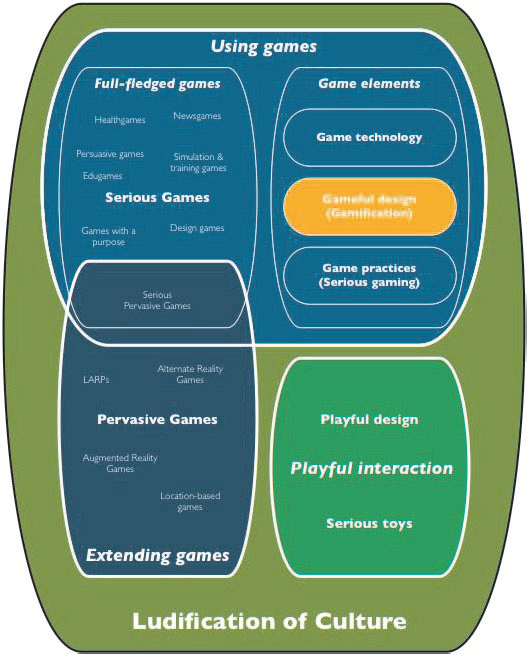
\includegraphics[width=100mm]{images/ch3_img02_gamification.png}
\caption{Gamification nach \textcite{Deterding.2011}}
\label{img:ch3_img02_gamification}
\end{center}
\end{figure}

Eine Einordnung und Abgrenzung der Terminologie ist in \ref{img:ch3_img02_gamification} zu sehen. \textcite{Deterding.2011} grenzen hierbei die Gamification als Prozess ab, der für die Erstellung der Spielelemente dient. Dieser Prozess wird verwendet um unter anderem Serious Games erstellen zu können. Diese stehen wiederum im Kontrast zu den Spielen zur normalen Unterhaltung, welche als Ausgangsbasis keinen alltäglichen Sachverhalt besitzen.

In der Literatur werden die Elemente Points, Badges und Leaderboards (PBL) angesprochen. Diese dienen als Mittel um eine Gamification durchführen zu können. 
Points stellen Punkte dar, die verwendet werden um einen Fortschritt des einzelnen Spielers darzustellen. Dies sind zum Beispiel Meilen in Vielfliegerprogrammen oder Statuspunkte beim Bonus Programm der Deutschen Bahn.

Bei Badges handelt es sich um Abzeichen, welche für bestimmte Errungenschaften an den Spieler vergeben werden. Ein Beispiel hierfür ist das Trainspotter Badge bei Foursquare, welches ausgestellt wird, wenn der Spieler in eine gewisse Anzahl von Bahnhöfen besucht hat. Die Badges sollen einen gewissen Status gegenüber den restlichen Spielern suggerieren.

Leaderboards sind klassische Ranglisten. Diese dienen dazu einen Wettbewerb unter den Spielern zu erzeugen. Es wird empfohlen nicht auf die klassische Top10 Liste zurückzugreifen, wie es bei vielen Spielhallen Automaten üblich ist. Stattdessen soll der Spieler zwischen Anderen platziert werden. Hierbei sind im Idealfall die Ränge über und unter dem Spieler dessen Freunde (vgl. Foursquare). Dies verhindert, dass der Spieler von überhöhten Punktzahlen abgeschreckt wird.

\textcite{Zichermann.2011} erweitern das Modell in dem Sie es um weitere Aspekte ergänzen und diesem Struktur verleihen.
Sie verwenden den Begriff SAPS. Dieser unterteilt sich in Status, Access, Power und Stuff (SAPS).
Das bekannte Points, Badges und Leaderboards der Literatur wird unter Status zusammengefasst wie in nachfolgender Aufzählung zu sehen.

\begin{itemize}
\item Status (Badges, Levels, Leaderboards)
\item Access (early Access)
\item Power (give power, e.g. modicum control over other players)
\item Stuff (give a reward, try to prevent that the price gets known)
\end{itemize}

Bei Access handelt es sich um \glqq Zugriff\grqq{} zu exklusiven Dingen, welche man dem Spieler gewährt. Ein Beispiel hier für ist die Lufthansa Senator Lounge oder die DB Lounge.
Es kann sich aber auch um einen zeitlich verfrühten Zugriff auf ein Produkt oder Funktionen handeln.

Unter Power sind Regeln zu verstehen, welche es dem Spieler erlauben Einfluss (Macht) auf andere Spieler auszuüben. Dies kann z.\,B. durch Moderationsrechte ab einem bestimmten Level realisiert werden. Foursquare realisiert dies durch Superuser.\cite{Lindqvist.2011}

Der letzte Punkt stellt Stuff dar. Es handelt es sich um Belohnungen die dem Spieler zuteilwerden. Klassischerweise handelte es sich z.\,B. um ein zusätzliches kostenloses Eis. Ziel ist es, dass dem Spieler nicht der konkrete monetäre Gegenwert ersichtlich wird. D.h. der Spieler soll nicht erkennen, wie viel seine Belohnung wert ist. Das Ziel sollte es nicht sein dem Spieler kostenlose Produkte zu geben, sondern etwas, was seinen Status unterstreicht.\\

Im Zuge der Gamification wird gerne der Begriff des Flow-Zustandes aufgegriffen.
Es handelt sich um einen von \textcite{Csikszentmihalyi.1991} eingeführten Begriff, bei dem es darum geht den Spieler zwischen einem optimalen Zustand zwischen Anspannung und Langeweile zu halten. Im Flow Modell wird angenommen, dass der Mensch sich in einer Situation jeweils seiner Handlungsmöglichkeiten und Fähigkeiten bewusst ist.
Übersteigt der Umfang der Aufgaben die Fähigkeiten, stellt sich ein Zustand oberhalb des Flow-Zustandes ein, wie in Abbildung \ref{img:ch03_img02_flow} zu sehen. Bei einer Unterforderung oder Einschränkung der Handlungsmöglichkeiten stellt sich schnell Langeweile ein. Das Ziel ist es den optimalen Zustand für den Spieler zu finden. Viele Spiele arbeiten unter anderem mit dynamischen Schwierigkeitsstufen, die berüchtigte Gummi-Band KI ist ein klassisches Beispiel.\cite{Bateman.2011}

\begin{figure}[H]
\begin{center}
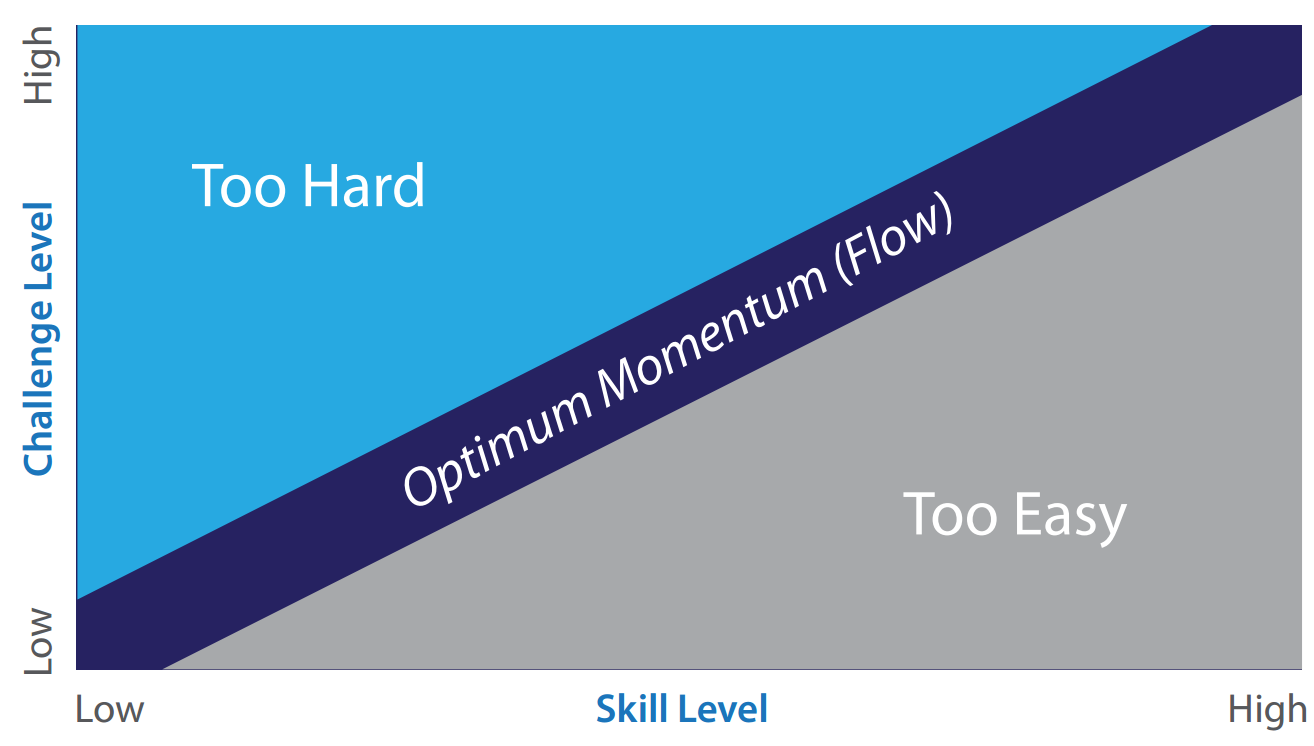
\includegraphics[width=120mm]{images/ch03_img02_flow.png}
\caption{Flow Zustand nach \textcite{Csikszentmihalyi.1991}}
\label{img:ch03_img02_flow}
\end{center}
\end{figure}

\section{Location-based Games}
\label{ch3:s:Geogames}

\subsection*{Spiel}

Für die Definition von Geogames, muss zunächst der Spiel-Begriff definiert werden. In der Literatur gibt es hierfür eine Vielzahl von Definitionen.
In dieser Arbeit soll die Definition analog zu \textcite{Salen.2004} verwendet werden, welche ein Spiel als Situation in Abgrenzung zum normalen Alltag darstellen. Ein Spiel wird innerhalb eines sogenannten Magic Circles durchgeführt, welcher das Spiel und die teilnehmenden Spieler von der Realität abgrenzt.
Dieser magische Kreis dient als Regelraum in welchem dann ein Spiel nach vorgegebenen Regeln durchgeführt wird. Im Kontrast stehen hier zu Alltagssituationen, wie das Einkaufen oder die Arbeit.

%\subsection*{Spielertypen}

\subsection*{Mobilegames}

Unter Mobilegames sind Spiele aller Art zu verstehen, die unterwegs gespielt werden. Diese werden auf mobilen Endgeräten gespielt.\cite{Bell.2006} Unter Mobile Endgeräte fallen klassische Handheld-Konsolen wie z.\,B. der Nintendo Game Boy und Smartphones.

\subsection*{Location-based Games}

Ortsbezogene Spiele werden in einem Geokontext gespielt werden. Hierbei wird die aktuelle Position des Spielers als Kontrollelement verwendet.\cite{Schlieder.2006} Durch dieses kann der Spieler mit dem Spiel interagieren.
Geogames sind eine Spezialisierung von ortsbezogenen Spielen, welche als Ursprung meist ein Brettspiel haben.
Geogames sind nicht begrenzt auf digitale Spiele, sondern haben Ihren Ursprung im Versteckspiel, auch in Form einer Schnitzeljagd. Ein späterer Nachfolger dieser stellt das Geocaching dar.\cite{Simanowski.2008}
Das Ziel der ortsbezogenen Spielen ist die Interaktion des Spielers mit der Umgebung. Dies unterscheidet sich von den klassischen Konsolen-Spielen, bei denen der Spieler das Spielgeschehen über einen Controller steuert. Grenzt man diese motorische Steuerung ab, gibt es die Zwischenstufe des Vistaspaces. Im Vistaspace steuert der Spieler das Spiel nicht mehr mit seinen Händen, sondern mit motorischen Bewegungen. Beispiele hierfür sind die Nintendo Wii und die Xbox Kinect. Bei diesen werden durch Lagesensoren und Infrarot Kameras die Bewegungen des Spielers erfasst und in die Spielsituationen eingebunden.
Findet das Spiel außerhalb eines Raumes statt, so wird vom sogenannten environmental space gesprochen.
Die Steuerung des Spiels und der Spielerposition findet durch Lokomotion statt.\cite{Benford.2003,Kiefer.2007}
Die drei kognitiven Räume beschreibt \textcite{Berendt.1999} in einer Gegenüberstellung der einzelnen Attribute.
\\\\
In der aktuellen Literatur werden vermehrt Spiele für Smartphones untersucht und entwickelt.\cite{Rashid.2006a}
Durch die Integration von GPS-Modulen, den fallenden Preisen für die mobile Datenübertragung und der Vereinfachung der Entwicklung der Spiele wächst auch die Zielgruppe.
\\\\
Eine Spezifizierung der ortsbezogenen Spiele stellen die sogenannten Geogames dar. Dieser Begriff wird vor allem von \textcite{Schlieder.2013} gepflegt. Es handelt es sich überwiegend um klassische Brettspiele, deren Spielkonzept auf ortsbezogene Spiele übertragen wird. Die Grundidee ist es, die strategischen Reize der Brettspiele mit den Affordanzen der Echtzeit Situation von ortsbezogenen Spielen zu verbinden. Dabei wird die rundenbasierte Spielmechanik ausgetauscht gegen die Lokomotion des Spielers. Die damit verbundenen Probleme und Schwierigkeiten werden in \textcite{Schlieder.2006} beschrieben.

\subsection*{Pervasive Games}

Unter Pervasive Games sind Spiele zu verstehen, welche den Magic Circle in seinen abgrenzenden Dimensionen erweitern.
Konkret werden die definierten Grenzen typischer Spiele überschritten.\cite{Montola.2005}
Es geht es um die Erweiterung der ortsspezifischen, zeitlichen und sozialen Grenzen.\cite{Montola.2009}
Darüberhinaus gibt es in der Literatur bei \textcite{Nieuwdorp.2007} und \textcite{Bjork.2007} eine weitere Dimension, welche als \glqq ambiguity 
of interaction or interface\grqq{} definiert wird. Dabei handelt es sich um die Unklarheit bzw. Eindeutigkeit der Interaktion.
Eine Vielzahl von Pervasive Games wurde in der Literatur behandelt und die Spielerinteraktion untersucht.
Beispiele hierfür sind Can You See Me Now \cite{Flintham.2003}, GeoTicTacToe, CityPoker, Neocartographer von \textcite{Schlieder.2005}, Human Pacman \cite{Cheok.2003} und Feed my Yoshi \cite{Bell.2006}.
Anhand dieser Spieler wurden Erkenntnisse in der Praxis gewonnen, welche sich mit der Gamification Literatur in Kapitel \ref{ch3:s:Gamification} decken.
Eine Sammlung weiterer interessanter Spielkonzepte stellt die Sammlung von \textcite{Hinske.2007} dar, welche Ideen für eigene Spielideen liefern kann.
Für die Umsetzung des Frameworks ist es wichtig einen Überblick und Einordnung über die aktuell existierenden Pervasive Games zu haben. Aufgrund dieser Informationen können bewusst bessere Entscheidungen im Entwurf getroffen werden, welche somit dem Spielleiter und dem darauf aufbauenden Spiel zugute kommen.


\section{Relokalisierungsansätze}
\label{ch3:s:Relokalisierung}

Ein wichtiger Aspekt im Zuge von Pervasive Games ist der Gamecontent. Soll ein Spiel außerhalb eines fest definierten Geografischen Raums durchgeführt werden, ist es notwendig fremde Umgebungen mit Inhalt zu füllen.\cite{Montola.2005} 
Bei der ortsbezogenen Relokation von Spielinhalten gibt es unterschiedliche Ansätze.
Zunächst müssen die ortsbezogenen Affordanzen beachtet werden. Hierbei handelt es sich um die lokalen Gegebenheiten, welche einen Einfluss auf das Spielgeschehen haben. Ein Beispiel hierfür sind Flüsse die ein Spielfeld teilen und damit die Distanz zwischen zwei einzelnen Spielelementen beeinflussen.
\\\\
Es gibt in der Literatur einen ersten Ansatz für die Relokalisierbarkeit von Spielfeldern.
\textcite{Kiefer.2005} beschreiben die Überlegungen bei der Durchführung des GeoTicTacToe Spiels in Bamberg. Bei der die Anordnung der 9 Spielpunkte einen Einfluss auf das Spielgeschehen hat. Brücken, Gebäude und Wege sind nicht strikt linear oder in Quadraten wie in vielen amerikanischen Städten oder z.\,B. in der Mannheimer Innenstadt. Für eine perfekte Ausgeglichenheit der Spielfelder müssten jegliche Informationen über Entfernungen, Fußgängerampeln Steigung des Wegs, körperliche Verfassung des jeweiligen Spielers, sowie dessen spatiale Fähigkeiten vorhanden. Dadurch entsteht ein äußerst komplexes Modell ohne Ideale Lösung. Daher wurden die ortsbezogenen Affordanzen als gegeben hingenommen bzw. in das Spiel als Herausforderung bzw. Spielelement integriert.

Generell gibt es drei Ansätze zur Relokation der Spielemente auf einer Karte.

\begin{itemize}
\item Keine Anpassung -- Spiel an einem Ort möglich
\item Komplette Anpassung -- Spiel an jedem Ort möglich
\item Hybride/teilweise Anpassung -- Spiel durch Eingriffe spielbar
\end{itemize}

In der Literatur werden die Probleme von ortsbezogenen Spielen öfters angesprochen, jedoch keine konkreten Lösungsansätze untersucht.
Die erste Möglichkeit stellen Spiele dar, welche keinerlei Anpassung enthalten.
Ein Beispiel hierfür ist REXplorer.\cite{Ballagas.2007} REXplorer ist nur in der Stadt Regensburg spielbar. Neben dem zugeschnittenen Geolocation Content ist der Controller explizit auf die Umgebung angepasst.
Hierbei handelt es sich um eine Art Zauberstab mit dem der Spieler mit den Elementen in der Umgebung interagieren kann. Diese Elemente sind jedoch explizit nur für die Stadt Regensburg erstellt worden und somit ist eine Funktion außerhalb nicht möglich.

Im Gegensatz dazu steht die zweite Möglichkeit. Es handelt sich dabei um Spiele, welche komplett ortsunabhängig gespielt werden können.
Dies kann entweder durch einen Algorithmus sicher gestellt werden oder durch die Tatsache, dass die Spielelemente keinen direkte Anpassung benötigen.
Spiele wie Feed my Yoshi, welche keine direkte Anpassung benötigen, haben deutliche Unterschiede im Hinblick ihrer Spielbarkeit abhängig von ihrer Umgebung. Die Autoren stellten  eine Korrelation zwischen Bevölkerungsdichte und Spielbarkeit fest, da die Spielelemente von WLAN-Accessspoints generiert wurden.\cite{Bell.2006}

Die letzte Möglichkeit stellt ein hybrider Ansatz dar. Bei diesem werden bestehende Spielfelder von einem vorgegebenen geografischen Kontext auf ein anderes Spielfeld übertragen. Hierbei wird unter Zuhilfenahme von Algorithmen ein Transfer der bestehenden Daten auf ein neues Spielfeld bewerkstelligt.
\\\\
Konkrete Lösungsansätze sind in der Literatur mit der Ausnahme von \textcite{Kiefer.2007}
nicht zu finden.
Der von \textcite{Kiefer.2007} gewählte Ansatz zielt darauf ab ein Vergleich von verschiedenen Spielfeldern herzustellen um Spieler von verschiedener Herkunft gegeneinander antreten können. Ziel ist es den Aufwand und die Kosten für die Durchführung dieser Spiele zu reduzieren. \textcite{Kiefer.2007} identifiziert drei Quellen die zu einer Heterogenität der Spielfelder führen:

\begin{itemize}
\item spatial scale -- Unterschied in geografische Größe
\item static structure -- Unterschied in geografischer Struktur (Straßen, Höhe) 
\item dynamic conditions -- Verändernde Gegebenheiten (Wetter, GPS/GSM-Empfang, Verkehr)
\end{itemize}

Eine gewisse Heterogenität der Spielfelder macht die Herausforderung für die Spieler interessanter. Zu große Unterschiede führen hingegen zu einem unfairen und damit weniger gutem Spielerlebnis.

Generell gibt es zwei Arten von ortsbezogenen Spielen. Zum einen örtlich begrenzte (spatial discrete) Spiele und zum anderen örtlich fortsetzende (spatial
continuous) Spiele.
Bei Ersterem handelt es sich um Spiele die auf einem abgegrenzte Spielfeld durchgeführt werden und die Position des Geocontents fest auf der Karte definiert ist. Letztere sind Spielfelder, welche unbegrenzte Spielfelder haben und die Spielinteraktion in jeder Position stattfinden kann.
Im Falle der spatial continuous Spiele ist ein bijectives Mapping der Orte nötig.
Bei einer Bijektion findet eine vollständige Paarbildung zwischen den Elementen vom Ursprungsspielfeld und Zielspielfeld statt.\cite{Athanasiadis.1999}
Dies funktioniert gut bei offenen Flächen. Bei der Verwendung von Straßen und innerhalb von Städten führt dies zu einer starken Verzerrung der Spielfelder und zu einer Diskrepanz zwischen Spielerfortbewegung und Lokomotion im Spiel.

Dies war der Grund, dass \textcite{Kiefer.2005b} spatial discrete Spiele im Detail untersucht haben.
Es wurde das Spiel CityPoker\cite{Kiefer.2005b} in zwei verschiedenen Städten gleichzeitig gespielt. Dabei konnten beide Teams der jeweiligen Städte über vordefinierte POIs miteinander interagieren. Untersucht wurde die optimale Gestaltung der Spielfelder zwischen den Städten. Zunächst wurden die POIs für beide Städte manuell nach eigenem Ermessen ausgewählt. Im Anschluss auf die Spielsitzung wurde untersucht, wie die unterschiedlichen Spielfelder ausgewählt werden müssten um ein optimales Feld zu erhalten. Hierbei ist zu beachten, dass die Reihenfolge der POIs bei Citypoker eine Rolle spielt.
Abbildung \ref{img:ch3_img03b_distributed} beschreibt ein ausgewähltes Spielfeld, sowie Distanzen zwischen den einzelnen Punkten.

\begin{figure}[H]
\begin{center}
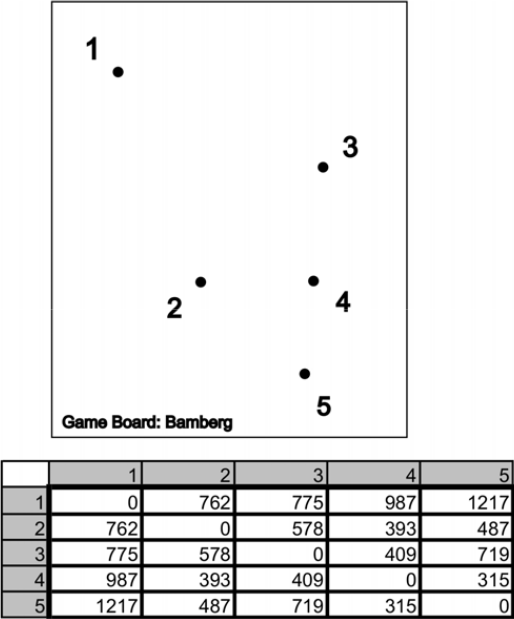
\includegraphics[width=100mm]{images/ch3_img03b_distributed.png}
\caption{Spielfeld Verteilung nach \textcite{Kiefer.2007}}
\label{img:ch3_img03b_distributed}
\end{center}
\end{figure}

Am Punkt 1 können Karten getauscht werden, welche beim anderen Team ebenfalls auf 1 liegen. \textcite{Kiefer.2007} stellen für den Vergleich  mehrere Entfernungsmatrizen auf, welche über ein Ähnlichkeitsmaß gegenüber gestellt werden.
Für die Berechnung der Ähnlichkeit wird nachfolgendes Maß angewandt:

\begin{equation}
similarity = \frac{1}{n} \sum_{row=1}^{n} \sqrt{ \sum_{col=1}^{n} (c_{1,row,col} - c_{2,row,col})^2 }
\end{equation}
\\
Hierbei stellen $c_1$ und $c_2$ jeweils die Entfernungsmatrizen der Spielfelder dar.
Row und col adressieren die Zeile und Spalte.
Zu beachten ist, dass die Entfernungen als direkte euklidische Luftlinie gemessen werden. Etwaige Höhenunterschiede, sowie örtliche Gegebenheiten werden aus Gründen der Vereinfachung nicht beachtet. Anschließend wird das arithmetische Mittel der Durchschnittswerte der einzelnen Reihen gebildet.
Als Ergebnis wird angenommen, dass spatial discrete Spiele eine einfachere Konfiguration erlauben wie unter anderem \textcite{Benford.2005} angemerkt haben.
\textcite{Benford.2005} identifizieren mehrere Herausforderungen im Bezug auf spatial continous games.

\begin{itemize}
\item Hefting domains
\item Configuration
\item Orchestration
\end{itemize}

Hefting domains stellen die Problematik dar, dass Spielelemente in Computerspielen auf die virtuelle Spielwelt fokussiert sind. Bei Pervasive Games muss dagegen ein besonderer Wert auf die Designentscheidungen bezüglich der virtuellen, reellen und hybriden Spielelemente gelegt werden.

Unter der Configuration ist die Adaption von Pervasive Games an verschiedene lokale Gegebenheiten zu verstehen. Darunter ist eine  (generierte) Erstellung von Spielfeldern an anderen Orten zu verstehen.

Die Orchestration stellt das Management des Spiels während der Laufzeit dar. Hierbei soll sichergestellt werden, dass ein Eingriff in das Spielgeschehen zu Gunsten der Sicherheit der Spieler als des Spielerlebnisses möglich ist.

Ein erster Ansatz für die automatisierte Relokalisierung von Spielfelder lässt sich in der Literatur bei \textcite{Mannara.2012} finden. Dieser entwirft am Beispiel von Uni Campi eine DSL\footnote{domain-specific language} zur Nutzung von OSM-Daten für das Auffinden von Spielelemente des gleichen Typs.
\\\\
Abschließend lässt sich feststellen, dass in der Literatur keine konkrete Lösung für die (teil-)automatisierte Erstellung von Spielfeldern existiert.
An dieser Stelle soll die Arbeit des Autors ansetzten und eine Lösungsmöglichkeit präsentieren.
Die daraus gewonnen Erkenntnisse sollen eine weitere Diskussion der Thematik ermöglichen.

\section{Verwendung offener Geodaten}
\label{ch3:s:offeneGeodaten}

Zunächst ist der Begriff offene (Geo-)Daten zu definieren.
Unter offenen Daten sind im folgenden Daten zu verstehen, welche unter freier Lizenz zur Verfügung stehen und somit ohne Lizenzgebühren verwendet werden können. Hierbei soll im Idealfall sowohl eine kommerzielle Nutzung als eine private Verwendung erfolgen können.
Es lassen sich generell zwei verschiedene Quellen von öffentlichen Geodaten identifizieren.
Als erste Möglichkeit gibt es Daten von öffentlichen Behörden. Es gibt aktuell im Zuge der Open Data Bewegung \cite{Oreilly.2007} den Anspruch Daten diverser Behörden den Bürgern zur Verfügung zu stellen. Der Grund liegt in der Argumentation, dass diese Daten mit Hilfe von Steuergeldern erstellt wurden. Erste Ansätze lassen sich sowohl in Großstädten wie Wien \cite{Wien.2014}, Hamburg \cite{Hamburg.2014} und Berlin \cite{Berlin.2014} finden. Als Beispiel für ganze Länder ist Dänemark \cite{Denmark.2014} zu nennen.\footnote{Eine Übersicht ist unter \url{http://www.engagedata.eu/opendatasites} (Abgerufen am 11.02.2014) zu finden. } Die Art, Qualität, sowie Umfang der Daten unterscheiden sich.
 
Die zweite Option sind offene (Geo-)Datenbanken, welche von privaten Personen durch manuelles Mapping oder externe lizenzierte Quellen zusammen getragen werden.
Beispiele für die Datenbanken sind OpenStreetMap (OSM)\footnote{\url{http://OpenStreetMap.org}} und Wikimapia\footnote{\url{http://wikimapia.org}}.
Hierbei stellt sich vor allem die Frage der Qualität der Daten im Vergleich zu kommerziellen bzw. Daten von Behörden.

\begin{figure}[H]
\begin{center}
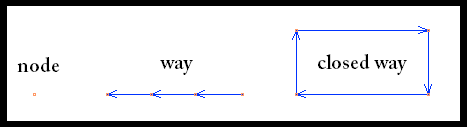
\includegraphics[width=120mm]{images/ch3_img03_OSM1.png}
\caption{OSM Elemente}
\label{img:ch03_img03_OSM1}
\end{center}
\end{figure}

Da für die Umsetzung des Frameworks OSM zum Einsatz kommen soll, ist eine Einschätzung im Hinblick auf die Anforderungen notwendig.
In Abbildung \ref{img:ch03_img03_OSM1} sind ein Teil der Standard Elemente von OSM zu sehen.
Generell werden alle Kartendaten durch Nodes, Ways und Relations dargestellt. Ways sind miteinander verbundene Nodes und Relations enthalten Relations, Ways, Nodes.
Für jeder der drei Typen können Tags zugewiesen werden. Damit können jedem Objekt mehrere Key-Value Paare zugewiesen werden, welche als Attribute zur Beschreibung der Objekte dienen.

In der Literatur haben sich viele Autoren mit der Qualität von OSM beschäftigt.
\textcite{Haklay.2010}, \textcite{Flanagin.2008} und \textcite{Goodchild.2007} beschreiben die Motivation der Personen die Kartenmaterial pflegen. Darüber hinaus wird auf die Probleme in offenen Datenbanken eingegangen. Es wird angemerkt, dass je nach Ziel des Mappers eine unterschiedliche Qualitätsstufe erreicht wird.
\textcite{Girres.2010} beschreiben in einem Vergleich von französischer Daten, dass die Qualität der Daten von OSM seit dem Beginn des Projektes in 2004 deutlich zugenommen hat. Auf dem Land gibt es im Vergleich zu Städten unterschiedliche Abdeckungsraten. Zudem haben Naturkatastrophen einen Einfluss auf die Qualität der Daten.\cite{Zook.2010}
Zur Zeit gibt es bei OSM ca. 25.000 aktive Mapper.\cite{OSM.2013} Die Autoren stellen eine Korrelation zwischen Einwohnerdichte und Datenqualität fest.
Die durchschnittliche Abweichung der Position beim Vergleich von OSM zu kommerziellen Kartenherstellern beträgt zwischen 1 und 30 Metern.
Darüber hinaus gibt es eine Ungenauigkeit bei Namen von Objekten. Diese entstehen unter anderem durch die Nutzung unterschiedlicher Sprachen und durch lokale Besonderheiten.
Die Einfachheit von OSM durch die Reduktion der Daten auf Nodes, Ways und Relations mit den dazugehörigen Tags hat den Nachteil, dass im Modell keine logische Konsistenz sichergestellt wird. Dies muss in der Verarbeitung der Daten berücksichtigt werden.
\textcite{Hecht.2013} beschreiben, dass eine geringe Abdeckungsrate im Vergleich zu professionellen Daten gibt. Dies wird ebenfalls von \textcite{Pfoser.2013} angemerkt. Diese weisen allerdings darauf hing, dass OSM eine hohe Klassifikationsrate besitzt. Zwar stellen die Autoren eine hohe Fehlerrate von bis zu 23\% fest, diese ist aber für den konkreten Anwendungsfall als Nutzung für Spielfelder  zu vernachlässigen.
\\\\
Für OSM gibt es im Vergleich zu Wikmapia ausgereifte Schnittstellen. Konkret sind zwei von Relevanz, die für eine Abfrage von Daten in Frage kommen.
Die erste Möglichkeit stellt die OSM API dar. Sie ermöglicht den Export der Geoinformatioenen bezogen auf eine Bounding Box. Eine detaillierte Filterung darüber hinaus ist nicht möglich.
Als zweite Möglichkeit gibt es die OSM XAPI (Extended Api). Hierbei ist es möglich Abfragen in Verbindung mit den zugehörigen Tags zu erstellen.\cite{Meyer.2013} Die Ergebnisse der Abfrage werden als XML-Dokument zusammengefasst.

Auf Basis der Literaturrecherche lässt sich daher schlussfolgern, dass OSM eine ausreichende Qualität für die Erstellung von Spielfeldern besitzt. Die Anforderung sieht nicht vor, dass alle Elemente erfasst werden, sondern nur sichergestellt wird, dass genügend Spielelemente vorhanden sind.



\section{Bewertung von Spielfeldern}
\label{ch3:s:geostatistik}

Für die spätere Bewertung der Spielfelder ist es notwendig passende Verfahren zu nutzen.
Hierfür eignen sich Verfahren der Geostatistik. Geostatistische Methoden haben ihren Ursprung in der Hydrologie.\cite{Bloschl.2006}
Das Ziel in der Geostatistik ist es geografische Daten zu analysieren und im besten Fall Interpolationen für unbekannte geografische Positionen zu bestimmen.\cite{Liebhold.1993}
Die Verwendung von Geoinformationssystemen (GIS) ermöglicht es hierbei Geodaten zu sammeln, speichern und wieder abzurufen. Gleichzeitig ist es möglich Daten zu transformieren und zu analysieren.\cite{Kitanidis.1997}
\textcite{Bailey.1995} definieren die statistische Analyse von Räumlichen Daten genauer und unterscheiden zwischen spatialen und nicht spatialen Analysen. Vergleicht man die Anforderung, dass eine Verteilung von Spiefeldern bzw. Spielelementen untersucht werden soll, so lässt sich feststellen, dass in der klassischen Literatur der Geostatistik weniger Ansätze zur Untersuchung von der Verteilung von Elementen auf einer Karte finden lassen.

Für die Evaluation der Spielfelder muss untersucht werden, wie die Spielelemente optimal verteilt werden müssen.
Da die Fortbewegung der Spieler sich auf Wege begrenzt muss daher die Literaturrecherche den Fokus auf die optimale Verteilung von Punkten in einem (Wege-) Netzwerk richten.
In der klassischen geostatistischen Literatur werden Verteilungen zunächst per Dichte unter Einfluss einer Zufallsvariablen beschrieben.\cite{Heinrich.1992}

Um ähnliche Aussagen über gewichtete Netzwerke machen zu könne, müssen die Methoden auf Netzwerke übertragen werden.
\textcite{Goovaerts.1997} beschreibt bei die Verteilung von Ressourcen in einfachen Histogrammen und Streudiagrammen, welche die Konzentration der Ressourcen beschreiben. Darüber hinaus besteht die Möglichkeit mit einem Kreisdiagramm die gewichtete Verteilung zu visualisieren.\cite{Diggle.2007}
Für die Visualisierung von Netzwerken zeigt \textcite{Okabe.2006} wie ein farbiges Voronoi Diagramm erstellt werden kann, welches als Charakteristik die nächsten entfernen Punkte beschreibt. \textcite{Spooner.2004} gehen einen Schritt weiter und definieren eine K-Funktion auf Basis von \textcite{Okabe.2001}, welche die Anzahl der Punkte in einem vorgegebenen Radius zu einem festen Punkt beschreiben.
Die Formel ist wie folgt definiert:

\begin{equation}
K(t) = \frac{1}{p}E(n_{pit})
\end{equation}
\\
E stellt der Erwartungswert in Hinblick auf p$_n$ dar. P beschreibt die Anzahl der zu untersuchenden Punkte und $n_{pit}$ beschreibt die Anzahl der Punkte die innerhalb der vorgegebenen Netzwerkdistanz t zum prüfenden Punkt p$_i$ stehen.
Dieser Ansatz soll als erste Evaluationsansatz der Spielfelder dienen, da er einfach zu berechnen ist und später angepasst und verbessert werden kann.



\newpage
\section{Lösungsansatz}
\label{sec:S4_Lösungsansatz}

\subsection{Mögliche Lösungen}

\subsection{Gewählter Lösungsansatz}

\newpage
\chapter{Umsetzung}
\label{ch:S5_Umsetzung}

\section{Erläuterung des Softwaretechnischen Entwurfs}
\label{ch5:s:Entwurf}

Für die Softwaretechnische Umsetzung wurden zunächst die Anforderungen an das Geogameframework in Kapitel \ref{ch4:s:Lösungen} sowie die gewählte Lösung aus Kapitel \ref{ch4:s:choosen_solution} im Detail evaluiert. Für die Umsetzung des Entwurfs wurde zunächst ein Entwurfs des Prozesses identifiziert, welcher die Geodaten aus OSM bis hin zur Darstellung im Beispiel Spiel darstellt. Eine Visualisierung ist in Abbildung \ref{img:ch5_img01_framework_progress} zu sehen.
\\\\

\begin{figure}[H]
\begin{center}
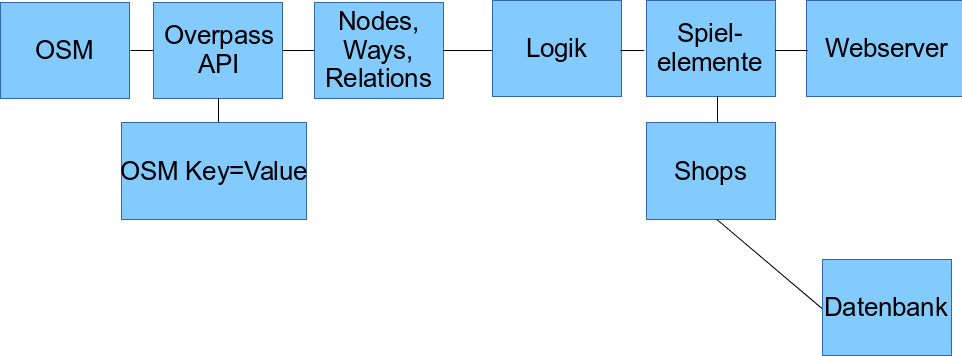
\includegraphics[width=140mm]{images/ch5_img01_framework_progress.png}
\caption{Prozess: Von OSM zum Spielelement}
\label{img:ch5_img01_framework_progress}
\end{center}
\end{figure}

\subsection*{OSM und Overpass API}

Zunächst steht zu Beginn des Prozess als Datengrundlage OpenStreetMap.
Die Daten werden allerdings nicht direkt von OSM über die OSM API abgerufen, sondern über Overpass. Das liegt daran, dass die OSM API selbst nur sehr rudimentäre Abfragen erlaubt.
Stattdessen wird die Overpass API verwendet, da diese geografische Abfragen erlaubt.\cite{Meyer.2013}
Diese Abfragen sind notwendig, für die Anforderung notwendig, da die Spielelemente basierend auf einem OSM Key-Value Paar ausgelesen werden sollen. Darüber hinaus wird die Transformation der Relations und Ways in Nodes einfacher ermöglicht.
Durch die Verwendung der Overpass QL-Abfrage Sprache (OQL) ist es möglich nicht nur die jeweiligen Relations, Ways und Nodes eines Tags zu erhalten, sondern auch zusätzlich alle rekursiv enthaltenen Elemente. Dadurch wird der komplette Datensatz mit einer Abfrage erhalten, der für die spätere Transformation benötigt wird. Der Vorteil liegt darin, dass nicht mehrere Abfragen gestartet werden müssen und somit die Zeit bis alle Daten zur Verfügung stehen erheblich reduziert wird. Die Overpass API selbst bietet diverse Ausgabe-Formate wie XML und JSON \cite{Olbricht.2014}. Für eine konkrete Umsetzung wurde sich bewusst für JSON entschieden. JSON bietet eine deutlich höhere Performance bei der Verarbeitung von JSON Dokumenten im Vergleich zu XML Dokumenten.\cite{Nurseitov.2009} Darüber hinaus ist das Zielformat GeoJSON und damit entfällt eine extra Transformation.
Der Aufruf der OverpassAPI erfolgt mittels einfacher REST-Abfrage:
\\\\
\url{http://overpass-api.de/api/interpreter?data=OQL_BEFEHL}
\\\\
Über den Parameter \glqq data\grqq{} wird der jeweilige OQL Befehl abgesetzt.
Für die Weiterverarbeitung der Daten wird im Anschluss das JSON Ergebnis vom Framework geparst und weiterverarbeitet.

\subsection*{Transformations Logik}

Die Transformation der Relations und Ways wird wie in Kapitel \ref{ch4:s:choosen_solution} umgesetzt. Eine Visualisierung ist in Abbildung \ref{img:ch5_img02_transform} zu sehen.

\begin{figure}[H]
\begin{center}
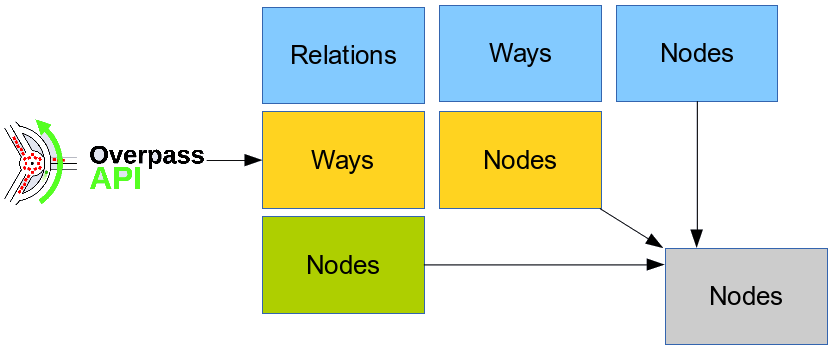
\includegraphics[width=140mm]{images/ch5_img02_transform.png}
\caption{Transformationsprozess: Relations, Ways, Nodes}
\label{img:ch5_img02_transform}
\end{center}
\end{figure}

Auf der linken Seite sind vertikal die Ausgangstypen angeordnet. Hierbei handelt es sich um die bereits angesprochenen Elemente Relations, Ways und Nodes. Im ersten Schritt werden die Daten der Overpass API aufbereitet. Im Anschluss werden alle Relations behandelt. Die Ways und Nodes, werden darauf bearbeitet. Hiermit sollen zunächst alle Ways und Nodes identifiziert werden, welche direkt einer Relation angehören und keine separaten Spielelemente darstellen. Die Vorgehensweise ist damit begründet, dass die Anzahl der Anfragen für ein Spielfeld auf eine reduziert wird. Somit enthält die Antwort alle Ways und Nodes. Die Nodes einer Relation, als auch die eines Ways, welche selbst nicht eigenständig sind werden zuerst ignoriert. Daher müssen die Elemente nacheinander, wie in Abbildung \ref{img:ch5_img02_transform} zu sehen, abgearbeitet werden.
\\\\
Zunächst werden alle Relationen identifiziert. Für jede Relation werden nun die beinhalteten Ways und Nodes identifiziert. Diese wiederum werden dann als \glqq gecalaimed\grqq{} markiert. Relations selbst werden nicht rekursiv aufgelöst, da es nicht das Ziel ist möglichst wenige Spielelemente zu haben, sondern die Relationen zu transformieren. Sollten Relations mehreren Unterrelations haben so sollen diese als Eigenständige Elemente betrachtet werden. Sollte dieser Ansatz sich als nachteilig in der Evaluation herausstellt, muss er entsprechend modifiziert werden.
Für die jeweilige Iteration eines Relation Elements werden  alle beteiligten Ways und Nodes zu einer Liste von Nodes zusammengefasst. Diese Liste wird wiederum durch das in Kapitel \ref{ch4:s:choosen_solution} beschriebene Verfahren auf ein virtuelles Node reduziert. Hierzu wird für die Bounding Box der Mittelpunkt berechnet, welche die Relation repräsentiert. Dieses virtuelle Node hat eine Koordinate, sowie eine ID welche es eindeutig identifizierbar ist. Hierzu wird die Relations ID von OSM verwendet.

Im nächsten Schritt werden die Ways abgearbeitet. Bereits als \glqq geclaimed\grqq{} markierte Ways, die somit bereits in einer Relation enthalten sind, werden ignoriert. Alle anderen Ways werden entsprechend jeweils wiederum zu einer Liste von Nodes und anschließend zu einem virtuellen Node transformiert. Hierbei entsteht wieder eine Koordinate und als ID wird die OSM Way ID verwendet.

Die als Node vorliegenden Elemente können direkt übernommen werden. Sie werden in Spielelemente, hier durch das graue Nodes Element symbolisiert, transferiert. Hierzu wird die Koordinate, sowie die OSM ID der Nodes übernommen.

Eine Problematiks tellt sich allerdings noch in der eindeutigen Identifizierung der virtuellen Nodes. Da diese von unterschiedlichen Elementen (Relatons, Ways, Nodes) abgeleitet wurden muss sichergesteltl werden, dass anhand der ID eine eindeutige OSM Zuordnung möglich ist.
Entweder es wird zusätzlich der abgeleitete typ des Spielelements explizit gespeichert oder aber, man transcodiert die Information mit in die ID.
Wenn man sich zunächst die OSM IDs für Nodes anschaut, stellt man fest, dass diese die 32bit signed Integer Grenze überschritten haben (Februar 2013). Im OSM Wiki wird daher empfohlen den Datentyp long zu verwenden, welcher in den Standard-Implementierungen ein 64bit Wert ist \cite{OSM.2013b}.
Eine Möglichkeit den Typ des Spielelements zu übertragen ist die Verwendung einer Bitmaske, welche den Typ in der ID codiert. Hierzu könnte man die den 2. und 3. Bit eines 64bit long Wertes verwenden. Der 1. Bit wird nicht verwendet um negative Zahlen weiterhin zu erlauben. Der 2. Bit würde als Identifikator für Relations dienen und der 3. für Ways als Ursprungselement. Ein Beispiel für den transformierten Way mit der OSM ID 1 ist in Abbildung \ref{img:ch5_img03_bitmask} zu sehen.

\begin{figure}[H]
\begin{center}
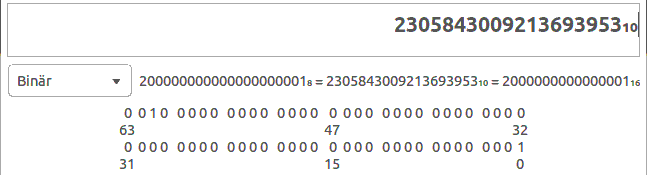
\includegraphics[width=120mm]{images/ch5_img03_bitmask.png}
\caption{OSM ID: Bitmaskenkodierung im 64bit long Wert}
\label{img:ch5_img03_bitmask}
\end{center}
\end{figure}


Wenn man die Reduzierung von 63bit (signed) auf 61bit(signed) mit der aktuellen Mapping Geschwindigkeit bei OSM vergleicht, so lässt sich feststellen, dass die Reduzierung um 2 bit aus Paradigmensicht zwar unsauber erscheint, aber eine Überschreitung der ID \begin{math}2^{61}\end{math} in ferner Zukunft liegt. Zudem könnte im Bedarfsfall wenn OSM auf 128bit IDs umsteigt die Bitmaske entsprechend angepasst werden.

\subsection*{Händler Integration}

Nachdem die virtuellen Nodes für die Spielelemente erstellt wurden, müssen die Elemente um die Händlern POIs ergänzt werden. In Kapitel \ref{ch4:s:choosen_solution} wurde erläutert, dass die Händler nicht als aktives Spielzielelement verwendet werden sollen, sondern eine Integration der Händler und Dienstleister im Spiel als Repräsentation ihrer selbst. Die Händler fungieren in diesem Zusammenhang als Anbieter für Items und andere Gegenstände. Für die spätere Darstellung auf der Karte müssen diese ebenfalls mit einer Koordinate versehen werden und separat behandelt werden. D.h. die Spielpunkte der Händler kommen stattdessen aus einer lokalen Datenbank. Dabei wird bewusst auf die Verwendung von OSM Als Basis verzichet. Zwar könnte man in einer erweiterten Version des Frameworks dem Nutzer unterstützen mit automatischen Vorschlägen basierend auf OSM, jedoch ist dies in der Grundfunktion nicht notwendig. Hier soll der Händler sich beliebig frei auf der Karte Positionieren können und entsprechende Parameter seines virtuellen Geschäfts festlegen. Im Anschluss soll er entsprechende Items in seinem virtuellen Shop hinterlegen können. Da die Items eventuell vom Händler gegen einen Betrag vom Spielleiter erkauft werden, hat der Spielleiter ein  Interesse an der Verwendung der Items im Spiel. Allerdings muss auch sichergesteltl werden, dass auf der anderen Seite das Spiel nicht in einen unausgeglichenen Zustand gerät. Wenn zu viele Spieler die Items eines Händlers bevorzugt werden, kann dies zu Frust bei den benachteiligten Spielern führen. Daher sollte es im Ermessen des Spielleiters liegen, dass dieser die Art und Verwendung der Items selbst definiert und entsprechende Vorschläge für die Händler parat hat. Dass der Händler sich selbst mit Spielmechaniken und Balancing auseinander setzt, ist höchst unwahrscheinlich und würde nur zu mehr Koordinationsaufwand führen. Daher ist es am sinnvollsten dem Händler gewisse Items mit standard Eigenschaften anzubieten. Von diesen wiederum kann er einen Typ auswählen und eine entsprechende Menge seinem virtuellen Shop zuordnen.
Für die Itemtypen kann der Spielleiter aller Voraussicht nach auf gewisse Grunderfahrungen zurückgreifen. Darüber hinaus sollte das Framework ihm in einer erweiterten Ausbauphase auch entsprechendes Feedback über die Verwendung und Nutzung der Items aufzeigen. Aufgrund dieser Informationen können dann Rückschlüsse auf das Balancing gezogen werden.

\subsection*{Persistenz}

Ein wichtiger Aspekt des Frameworks stellt die Persistenz dar. Es müssen die Spielelemente, sowie der Spielzustand selbst gespeichert werden. Die Daten für die Spielelemente stammen aus OSM und von der lokalen Datenbank. Da die OSM Daten entsprechend transformiert werden, stellt sich die Frage ob dieser Prozess beschleunigt werden kann, wenn die Daten entsprechend in der Datenbank lokal zwischengespeichert werden.
In Kapitel \ref{ch4:s:choosen_solution} ist bereits auf diesen Aspekt eingegangen worden. Die Problematik die sich durch eine Zwischenspeicherung stellt ist zum einen die Aktualisierung der Daten. Die lokalen Daten müssten mit einem Zeitstempel versehen werden und gehalten werden, bis diese \glqq verfallen\grqq. Darüber hinaus müssten diese nach dem Verfallszeitpunkt entsprechend gelöscht oder aktualisiert werden oder belassen werden. Ein Caching kann sinnvoll sein, sofern das Framework für ein Spiel mit einer kritischen Masse an Spielern verwendet wird. Allerdings ist eine Evaluation und Untersuchung des Frameworks auf Hochskalierbarkeit nicht Bestandteil der ersten Ausbaustufe. Ein weiterer Aspekt stellt die Datenmenge dar. Sofern im Framework alle abgefragten OSM Daten in der Datenbank hinterlegt werden, ohne dass diese eine Zustandsveränderung erfahren haben, ist dies zwar modelltechnisch korrekt, allerdings aus Performance und Platzgründen nicht zu empfehlen.
Da das Framework dem Spielleiter so wenig Aufwand wie möglich machen soll, sollte verhindert werden, dass der Spielleiter sich um Datenbank und Speicherplatz Probleme kümmern muss. Ein gutes Beispiel hierfür stellt auch das OSM Projekt selbst dar. Die bekannte Kartendarstellung verwendet zur Anzeige entsprechende Tiles. Diese Tiles werden auf Basis der OSM Daten gerendert. Ein erster Ansatz wäre das Rendern alle Tiles.
Allerdings dauert der Renderprozess mehrere Tage und Aktualisierungen auf der Karte würden immer nur mit mehreren Tagen Verzögerung angezeigt werden. Hinzu kommt die Tatsache, dass nur ein Bruchteil der Kartendaten auch tatsächlich angeschaut wird (<2\% \cite{Haklay.2008}). Daher werden die Karten-Bilddaten in Echtzeit gerendert und nach einer gewissen Zeit wieder verworfen.
Daher ist es auch beim Framework nicht sinnvoll alle Daten zu speichern, sondern nur die Spielelemente mit denen ein Spieler aktiv interagiert hat.
Die Daten der Händler werden separat gespeichert. Sie befinden sich ebenfalls in einer Datenbank, besitzen allerdings im Vergleich zu den Spielelementen eine Persistenz unabhängig von ihrer Interaktion mit den Spielern.


\subsection*{Schnittstellen}

Ein Framework benötigt entsprechende Schnittstellen über die es Funktionen und Daten nach Außen hin zur Verfügung stellt. Zunächst muss geklärt werden, wie die Daten verwendet werden sollen. Für das Beispiel Spiel ist die Darstellung der Karte über eine Website vorgesehen. Unabhängig von der später verwendeten Technologie müssen in diesem Fall sowohl die Spielelemente, als auch die Händlerdaten vom Framework zur Verfügung gestellt werden.

Zur Verdeutlichung wird an dieser Stelle die Entscheidung für eine Technologie in Abbildung \ref{img:ch5_img04_interfaces} auf das nachfolgende Kapitel verlegt.

\begin{figure}[H]
\begin{center}
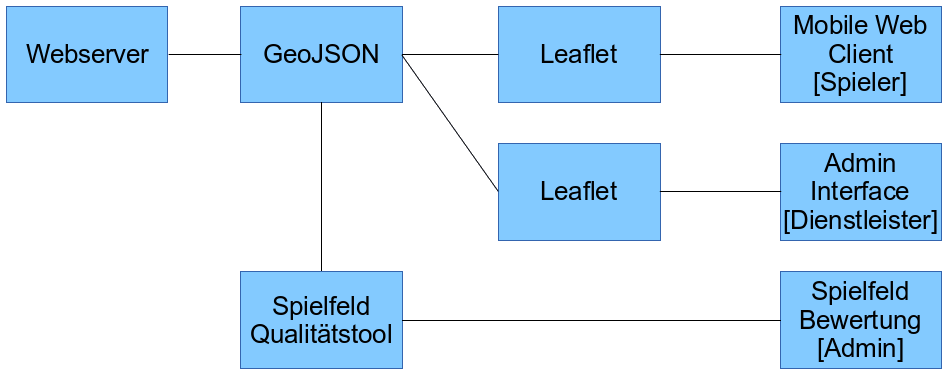
\includegraphics[width=140mm]{images/ch5_img04_interfaces.png}
\caption{Visualisierte Schnittstellen des Frameworks}
\label{img:ch5_img04_interfaces}
\end{center}
\end{figure}

Die Wahl des Formats für den Export der Spielelemente und Händlerdaten ist auf GeoJSON gefallen.
Dies ist mit den Daten von OSM/Overpass welche als JSON im Framework ausgelesen werden begründet. Darüber hinaus verwendet eine Vielzahl der aktuellen Frameworks und Tools dieses Format. Während das offene Format WKT für die reine Repräsentation von Geodaten dient \cite{Stolze.2003}, bietet das GeoJSON Format zusätzlich die Möglichkeit entsprechende Properties an ein Geo Objekt zu speichern \cite{Butler.2008}. Über diese kann wiederum das Framework Informationen wie z.\,B. die codierte OSM ID und Informationen zum Spielelement übertragen.
\\\\
Generell werden die Informationen des Frameworks für drei verschiedene Module benötigt.
Zunächst einmal gibt es den Spielclient bzw. dessen Oberfläche. Dieser benötigt die Daten für das Staging des Spiels selbst.
Über die Spieloberfläche interagiert der Spieler mit dem Spiel. Er sieht die aktuelle Karte, sowie die darauf platzierten Objekte. In diesem Fall sind dies die Spielelemente sowie die einzelnen Händler. Die Spielelemente selbst stellen im Beispiel Spiel die sogenannten Prestige Flaggen dar.
Ein weiteres Modul stellt die Administrationsoberfläche dar. Diese dient dazu dem Spielleiter sowie dem jeweiligen Händler eine Konfiguration des Spiels vorzunehmen. Im Detail kann der Spielleiter die entsprechenden Spielitems definieren, neue Händler anlegen und diese auf der Karte positionieren. Der Händler kann seine Metadaten pflegen und entsprechende Items, welche er in seinem virtuellen Laden anbieten möchte selektieren und anbieten. Bei Fehlern oder Aktualisierungen kann der jeweilige Administrator (Spielleiter oder Händler) diese problemlos anpassen. Für die Positionierung der virtuellen Läden auf der Karte wird ebenfalls analog zum Spielfeld eine GeoJSON Schnittstelle zum Einsatz kommen.
Das letzte Modul stellt die Evaluierung der Spielfelder dar. Hier wird dem Spielleiter durch die Verwendung der gleichen Schnittstelle, wie für die Aufbereitung des Spielfeldes, die Möglichkeit geboten Daten in ein entsprechendes Evaluationstool mit entsprechendem Algorithmus  zu importieren. Dieses Tool wird entsprechend in Kapitel \ref{ch:CH6_qualtiy_of_gameboards} in vorgestellt. Über dieses wird das ideale Key-Value Paar für die OSM Tag Selektion der Daten evaluiert. Dies soll dem Spielleiter die Möglichkeit einer Objektiven Bewertung der Spielfelder ermöglichen.

\subsection*{Darstellung}

Da das Framework für ortsbezogene Spiele verwendet werden soll, ist es daher unerlässlich dem Spieler, sowie den Administratoren eine entsprechende Visualisierung zu bieten. Zunächst gibt es das Spielfeld. Das Spielfeld verwendet im Hintergrund Kartenmaterial von OSM, auf das die einzelnen Elemente platziert werden. Die Karte selbst wird initial auf die (GPS-)Korrdinaten der Spielerposition zentriert. Dadurch ist es dem Spieler möglich sich direkt von seiner Position aus zu Orientieren. Die auf der Karte eingezeichneten Elemente wie Flaggen und Händler kann der Spieler somit problemlos identifizieren und zu Fuß aufsuchen. In Abbildung \ref{img:ch5_img05_dialog} ist ein Mockup der Kartenoberfläche zu sehen. Je nach Flaggenstatus werden die Flaggen unterschiedlich farbig dargestellt. Das Ziel ist es neutrale Flaggen grau, feindliche Rot und eigene grün darzustellen. Damit erhält der Spieler automatisch einen Überblick über die Situation und kann auch durch das Herauszoomen der Karte seine weiteren Spielzüge entsprechend planen.
Neben den Spielelementen werden dem Spieler die aktuellen Punkte angezeigt. Dieser wird im Beispiel Spiel durch das einfache Addieren der Prestige der Flaggen die im Spielerbesitz sind berechnet. Des weiteren wird dem Spieler eine Auswahl für sein Inventar angezeigt werden.
Über dieses kann er sich nicht nur alle Items in seinem Besitz anzeigen lassen, sondern auch diese verwenden. In einem späteren Ausbau des Frameworks sollen darüber hinaus Items mit anderen Spielern getauscht werden können.
Sofern der Spieler mit einer Flagge interagiert, wird ihm die aktuelle Prestigezahl der Flagge angezeigt. Je nachdem ob ihm die Flagge bereits gehört oder diese einem fremden Spieler angehörig ist, kann der Spieler diese \glqq angreifen\grqq. Durch den Angriff werden die Aktionspunkte des Spielers auf die Flagge transferiert. Ist die Flagge im Besitzt eines anderen Spielers so sieht der Spieler dies durch die aktuelle Farbgebung und kann durch den Einsatz seiner Aktionspunkte die Prestigezahl reduzieren, was direkt angezeigt wird. Für die Interaktion mit den Händlern steht dem Spieler ein Menü zur Verfügung. Dieses erscheint sobald der Spieler auf einen Händler klickt. Danach öffnet sich ein Menü über das der Spieler eine Übersicht der verfügbaren Items sowie deren Spielpreise erhält. Sollte der Händler Items, wie in Kapitel \ref{ch4:s:choosen_solution} beschrieben Coupons anbieten, so kann der Spieler diese an gegebener Stelle eingeben.

\begin{figure}[H]
\begin{center}
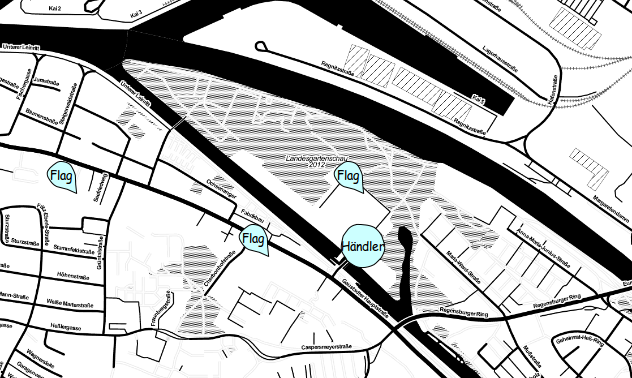
\includegraphics[width=140mm]{images/ch5_img05_dialog.png}
\caption{Spielfeld Mockup}
\label{img:ch5_img05_dialog}
\end{center}
\end{figure}

Der Administrationsbereich für den Spielleiter und den Händler arbeitet separat vom Spielfeld.
Je nachdem, ob Items oder Händler im System gepflegt werden sollen, wird dem Benutzer eine passende Liste präsentiert.
Beim Items Menü erhält der Benutzer eine Übersicht über alle Items die dem Spiel zur Verfügung stehen. Hierbei handelt es sich allerdings nicht um Item-Typen sondern direkt um die instantiierten Items selbst. Die Idee dahinter ist es, dem Spiel die Möglichkeit zu bieten auch einzigartige Items zu enthalten und sicherzustellen, dass ein Item jeweils auch immer als solches im System behandelt wird. Über die Liste gibt es die Option die bestehenden Items zu modifizieren oder zu entfernen. Neue Items können über eine Schaltfläche entsprechend angelegt werden. Dabei wird dem Benutzer eine entsprechende Oberfläche präsentiert und über Metadaten das Item genauer spezifiziert. Beispielsweise der Name, Itemtyp und der dafür  zu zahlende Preis.
\\\\
Möchte der Benutzer dahingegen Händler pflegen, so erhält er zunächst analog zu den Items eine Übersicht der einzelnen Händler.
Diese kann er analog zu den Items entsprechend modifizieren und löschen. Das Anlegen eines neuen Händlers ist genauso aufgebaut wie bei den Items. Der Unterschied liegt jedoch drin, dass es sich bei den Händlern nicht um einfache Formularfelder handelt, sondern auch zusätzlich eine Georepräsentation stattfinden muss. D.h. es muss die Positionierung des Händlers auf einer Karte erfolgen. Hierzu wird eine Art \glqq Picker\grqq{} verwendet. Auf einer OSM Karte soll der Benutzer die Position des Händlers definieren. Für eine Korrektur der Position reicht es aus, wenn der Benutzer einfach den Marker auf der Karte mit der Maus ergreift und per drag n drop auf seine neue Position bewegt.

%%\subsection*{Sonstige Funktionalitäten}


\subsection*{Technischer Entwurf}

Nachdem die Anforderungen beschrieben wurden, muss der Softwareteschnische Entwurf konkretisiert werden.
Um die Software entsprechend abzubilden zu können muss zunächst ein Modell entworfen werden, welche die Software abbildet. Die Prozesse des Frameworks wurden bereits in Abbildung \ref{img:ch5_img01_framework_progress} sowie \ref{img:ch5_img04_interfaces} visualisiert.

Zu Beginn einer Systementwicklung müssen die Usecases und die beteiligten Akteure identifiziert werden.
Hierfür wurde zu Beginn überlegt, welche Personen Zugang zum System haben sollen und welche Aufgaben diese am System erfüllen.
Dadurch wird sichergestellt, dass alle Aspekte behandelt werden, nicht nur die im initialen Lösungsansatz. Diese sind wichtig für den späteren Entwurf des Systems, sowie deren Umsetzung.
Die Usecases lassen sich als Diagramm wie in Abbildung \ref{img:ch5_img06_usecases} sichtbar definieren.



\begin{figure}[H]
\begin{center}
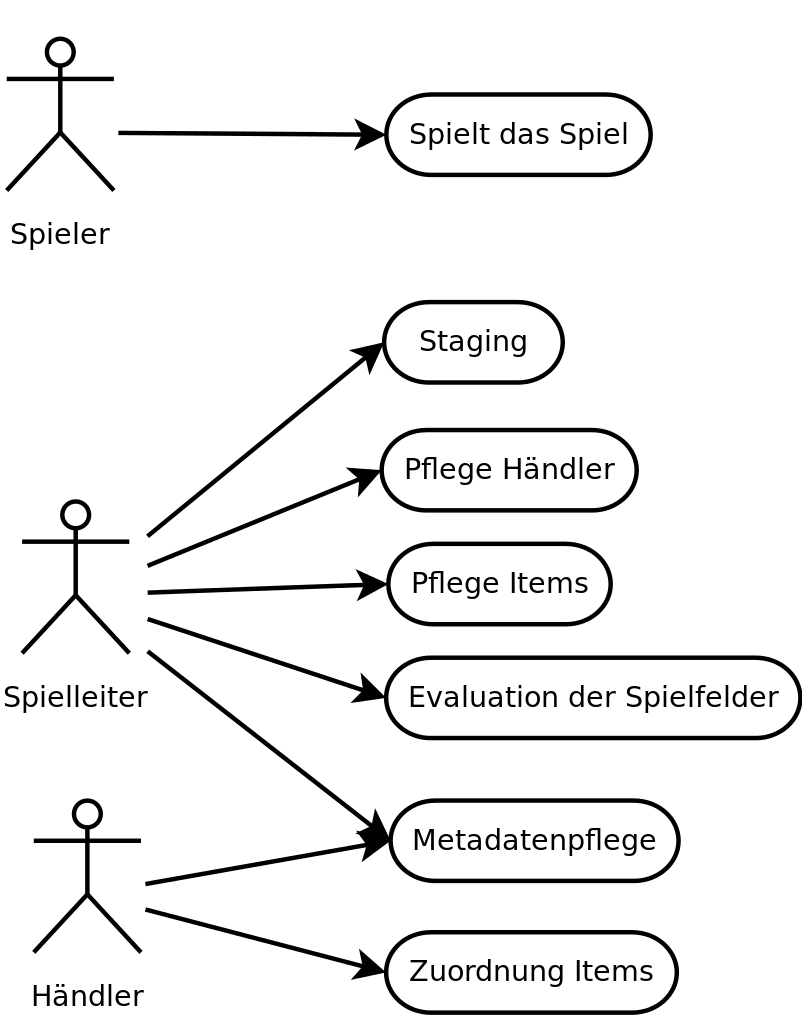
\includegraphics[width=100mm]{images/ch5_img06_usecases.png}
\caption{Usecase Diagramm}
\label{img:ch5_img06_usecases}
\end{center}
\end{figure}

Zunächst lässt sich feststellen, dass es drei Akteure gibt.
Diese decken sich soweit mit dem Lösungsansatz.
Der Spiele hat das Ziel das Spiel zu spielen. Der Spielleiter hingegen sieht es vor entsprechend das Staging des Spiels mit dem Framework zu bewerkstelligen.
Hier muss er die Händler als auch Items pflegen. Darüber hinaus teilt er sich mit dem Händler die Metadatenpflege, da je nach Situation der Spielleiter mehr oder weniger in die individuelle Pflege der Händlerdaten eingebunden ist. Der Händler möchte zusätzlich seine Items, die er vom Spielleiter zugewiesen bekommen hat entsprechend auf seine virtuellen Läden verteilen. In der Grundfunktion des Framesworks sind nur diese Benutzer vorgesehen. In einer zweiten Ausbaustufe des Frameworks ist es sinnvoll explizite Nutzerrollen einzuführen um eine detailliertere Rechtezuweisung zu ermöglichen.
\\\\
Durch die Verwendung einer objektorientierten Programmiersprache ist es notwendig entsprechende Klassen zu definieren.
Diese dienen dazu, Objekte abzuleiten und die jeweiligen Methoden von diesen zu nutzen.
Es muss sichergestellt werden, dass die Beziehungen zwischen den Klassen modular sind, damit ein einfacher Zugriff und eine Austauschbarkeit gegeben ist.
Um einen Einblick in die Struktur des Frameworks zu erhalten wird in diesem Abschnitt kurz auf die wichtigsten Aspekte eingegangen.


\begin{figure}[H]
\begin{center}
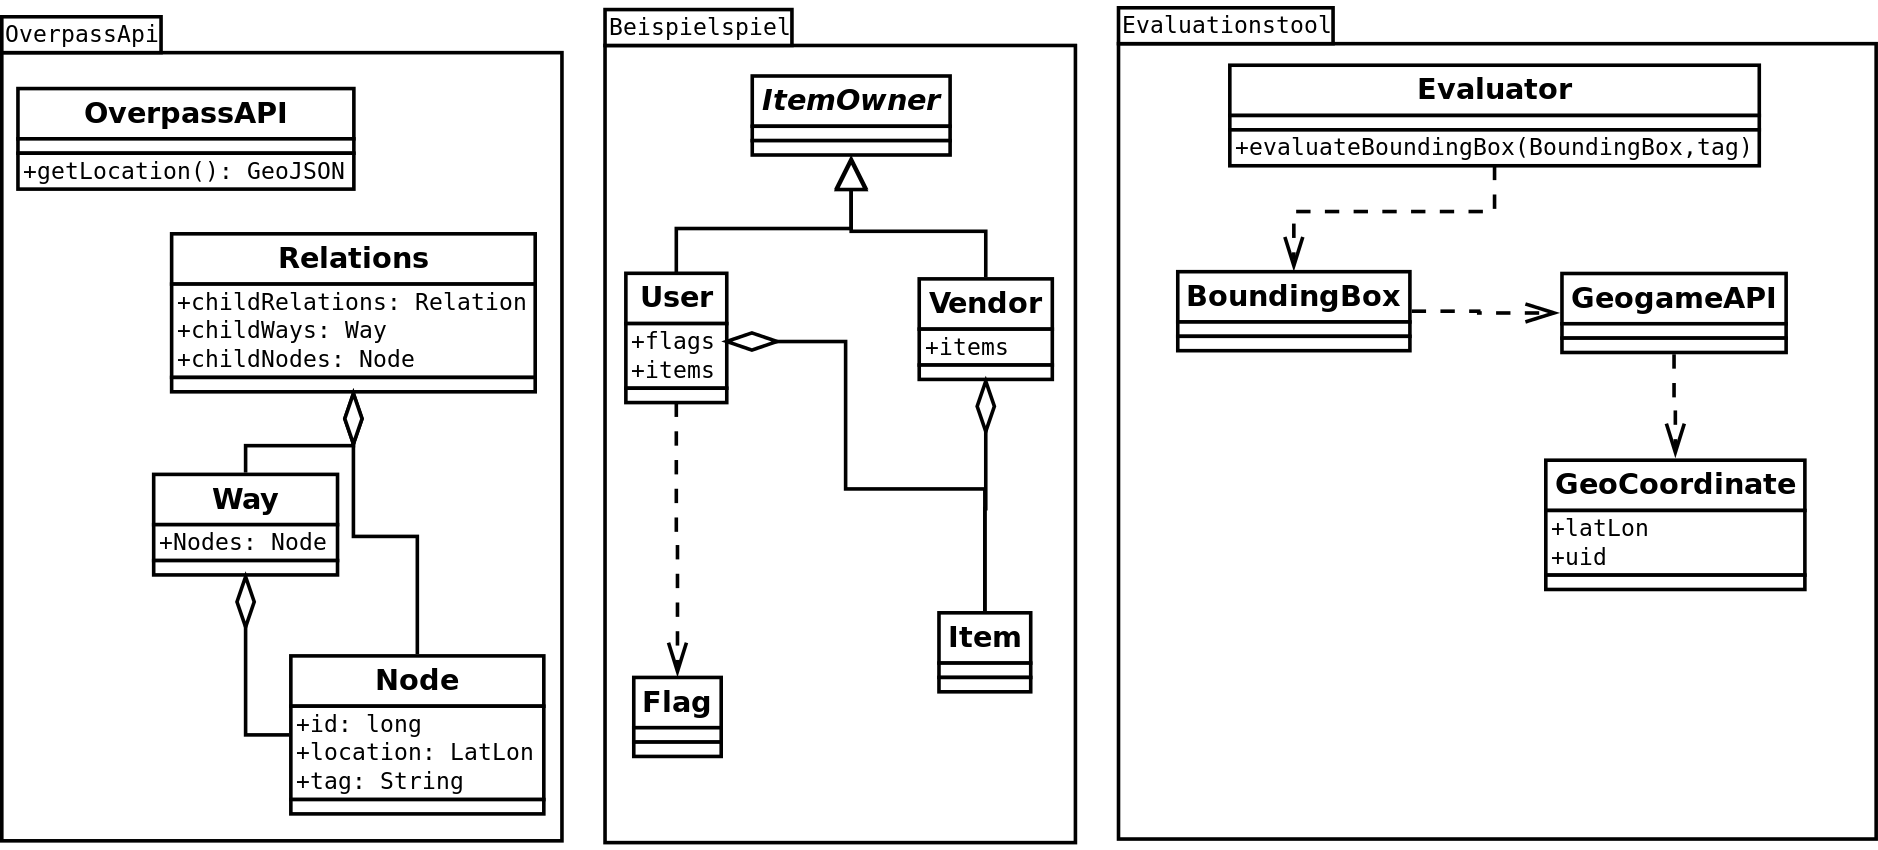
\includegraphics[width=150mm]{images/ch5_img07_classes.png}
\caption{Vereinfachtes Klassen Diagramm}
\label{img:ch5_img07_classes}
\end{center}
\end{figure}

In Abbildung \ref{img:ch5_img07_classes} ist ein vereinfachtes Klassendiagramm des Frameworks zu sehen. Das Framework als solches besteht aus drei Modulen. Zunächst gibt es den Bereich \textit{OverpassApi}. Hierbei handelt es sich nicht um die OverpassApi selbst, da Overpass selbst nur eine Webschnittstelle ist. Die beschriebene API ist die Implementierung einer entsprechenden Schnittstelle im Framework selbst. Sie liefert das Ergebnis der OverpassApi transferiert von den einzelnen Elemente Relations, Ways und Nodes. Diese werden wiederum durch den bereits beschriebenen Ansatz entsprechend transformiert in dem eine Umcodierung in virtuelle Nodes erfolgt. Im gleichen Zug wird überprüft, ob es persistierte Daten für die virtuellen Nodes in der lokalen Datenbank gibt. Sind entsprechende Daten vorhanden, so werden die virtuellen Nodes um die entsprechenden Properties ergänzt und anschließend als JSON bzw. GeoJSON ausgegeben.
Im Anschluss werden diese über die Webschnittstelle des eigenen Frameworks ausgegeben.
Für die Händler gibt es eine separate Schnittstelle im Framework, welche analog zur Overpass Implementierung fungiert, aber hierbei nicht die Daten von extern (OSM/Overpass) bezieht, sondern direkt in der fertigen Form aus der lokalen Datenbank auslesen kann. Hierbei ist zudem auch keine entsprechende Transformation notwendig, sondern diese liegen bereits als fertige Nodes vor. Dies ist möglich, da jeder Händler nur als einziger Punkt im Spiel repräsentiert wird.
\\\\
Das nächste Modul ist das Beispiel Spiel. Das Beispiel Spiel selbst wurde einfach gehalten, da es zum einen als Proof of Conecept des Frameworks dienen soll, zum anderen der Fokus auf die Verteilung der Spielelemente auf dem Spielbrett untersucht werden soll.
Es gibt 4 verschiedene Objekte. Spieler, Händler, Flaggen und Items.
Spieler und Händler stehen in einer polymorphen Verbindung zu Item. Beide Klassen leiten von einer abstrakten Klasse ItemOwner ab, welche entsprechende Methoden vorhält die für die Interaktion als ItemOwner essentiell sind. Beispielsweise der Verkauf oder die Benutzung eines Items. Ein Item kann nur einem Spieler oder einem Händler angehören, niemals aber beiden gleichzeitig. Es gibt darüber hinaus die Möglichkeit, dass ein Item ohne ItemOwner existiert. Ein Beispiel könnte es sein, dass der Spielleiter für ein Event bestimmte Items auf der Karte ablegt oder lokale zwei Spieler Items manuell tauschen möchten.
\\\\
Das letzte Modul stellt das sogenannte Evalutationstool dar.
Mit diesem sollen die erzeugten Spielfelder analysiert und bewertet werden. Eine genauere Erläuterung ist in Kapitel \ref{ch:CH6_qualtiy_of_gameboards} zu finden.
Das Evaluationstool gereift zunächst auf die GeoJSON Schnittstelle des Frameworks zu. Dieses liefert bei entsprechender Abfrage mittels Bounding Box und entsprechendem OSM Tags die Spielelemente zurück. Die Bounding Box wird auf Basis einer initialen Koordinate berechnet. Somit kann der Spielleiter einfach zwei Koordinaten definieren zu denen er gerne eine entsprechende Auswertung interessanter Tags erhalten möchte. Das Evaluationstool startet im Anschluss den Vorgang und wandelt die Spielelemente in vereinfachte Objekte mit ID und Geo-Kooridnaten um. Diese wiederum werden der jeweiligen Evaluationsmethode als Liste übergeben und deren Rückgabewert beschreibt die Kombination aus Bounding Box und OSM Tag.

\subsubsection*{Datenbank}

Aufgrund der vorherigen Analysen wird normalerweise ein Entity-Relationship-Modell (ERM) erstellt. Allerdings soll der Einsatz eines Webframeworks erfolgen, welches ein Objektrelationales Mapping unterstützt und somit die Manuelle Erstellung der Datenbankstruktur nicht vorgesehen ist. Dies wird unter der Annahme gemacht, dass das Framework später im Produktiv-Betrieb für die Datenspeicherung optional auf eine NoSQL Lösung umgestellt werden kann. Diese bieten eine bessere Performance bei einfachen Abfragen.
Dies geschieht vor dem Hintergrund den, in der Literatur häufig kritisierten, Mismatch zwischen objektorientierter Programmierung und Verwendung von relationalen Datenbanken zu entgegnen.\cite{Cattell.1991}

Die geringe Verbreitung der objektorientierten Datenbanken liegt darin, dass nicht
versucht wurde die bestehenden Datenbanken zu ersetzten.Stattdessen sind die bereits existierenden Datenbanken in Unternehmen nicht in neue objektorientierte Datenbanken transferiert worden. Der Grund hierfür liegt in den historisch gewachsenen Applikationen und Datenbanken, deren Umstellung einen sehr hohen Aufwand darstellen würde.\cite{Burleson.1994}

Ein weiter Aspekt ist die Tatsache, dass die objektorientierten Datenbanken nicht in jedem Aspekt
besser sind als relationale Datenbanken. Es gibt Situationen in denen besitzen objektorientierte
Datenbank Management Systeme klare Vorteile gegenüber den relationalen Datenbanken.
Die objektorientierten Datenbanken spielen ihre Vorteile speziell bei der Abbildung von Beziehungen von Objekten untereinander aus. Bei einer sequentiellen Abfrage mehrerer Datensätze sind
jedoch die Relationalen im Vorteil.\cite{Van.2006} Hier ist es notwendig den Zweck der zu speichernden Daten bzw. deren Verwendung zu untersuchen. Je nachdem kann der Einsatz von objektorientierten Datenbanken oder relationalen Datenbanken sinnvoll sein.

Vergleicht man die Verbreitung von objektorientierten Datenbanken in gewissen Einsatzgebieten, so lässt sich feststellen, dass diese trotz der in Summe geringen Verbreitung ein berechtigtes Dasein haben. Speziell in Geoinformationssystemen spielen objektorientierte Datenbank Management Systeme ein wichtige Rolle.\cite{Brinkhoff.2005} Diese können deutlich einfacher komplexe Verbindungen zwischen den unterschiedlichen Objekten herzustellen und ermöglichen eine Veränderung dieser Beziehungen in einem Bruchteil der Zeit. Die umfangreiche Literatur zum Thema Geoinformationsysteme gibt einen Ausblick für Möglichkeiten die sich durch die Nutzung dieser ergeben können.

\subsection*{Weitere Aspekte}

Ein weiterer Aspekt stellt die Optimierung der Anfragen an die Overpass Api Schnittstelle des Frameworks seitens des Spielfeldes dar. In der Grundvariante des Frameworks stellt das Spielfeld jeweils eine Anfrage als Bounding Box an die Schnittstelle um die aktuellen Spielelemente für den jeweiligen Kartenausschnitt zu erhalten. Eine Optimierung dessen wäre die Verwendung von dynamischen erweiterten gecachten Bounding Boxen. Das bedeutet, dass bei einer Abfrage zunächst die Bounding Box am Rand um jeweils X\% erweitert wird. Die zusätzlichen abgefragten Spielelemente werden allerdings nicht direkt angezeigt. Bewegt der Spieler nun das Spielfeld wird überprüft ob der aktuelle Kartenausschnitt sich noch innerhalb der dynamisch erweiterten Bounding Box befindet. Ist dies der Fall, so spart sich das Spiel einen zweiten Request. Dies hat zweierlei Vorteile. Der erste stellt eine Reduzierung der HTTP Request auf der Clientseite dar. Speziell bei ortsbezogenen Spielen ist der Empfang beim Spielen öfters eingeschränkt und nur GPRS oder EDGE seitens Mobilfunkanbieter verfügbar. Durch die Reduzierung der Reuqests wird die Spielperformance verbessert. Ein anderer Aspekt ist die Reduzierung der Anfragen auf der Server Seite. Es verbessert deutlich die Skalierbarkeit und ermöglicht somit mehr Spieler mit einem einzigen Server bedienen zu können.

%% performance messungen?

\section{Bewertung der Technologien und Werkzeuge}

Nachdem der Softwaretechnische Entwurf erstellt wurde, muss untersucht werden welche Technologien und Werkzeuge für die Umsetzung des Frameworks am besten geeignet sind.
Zunächst stellt sich die Frage in welcher Programmiersprache das Framework umgesetzt werden soll. Diese Frage lässt sich anhand der Anforderungen eingrenzen. Zunächst muss eine Website erstellt werden, welche ein Staging des Beispiel Spiel erlaubt und gleichzeitig die Spieldaten über eine Webschnittstelle exportieren kann. Hiermit lässt sich die Auswahl auf diverse Sprachen reduzieren, welche eine Erstellung dynamischer Webseiten erlauben.
Die nachfolgende Aufzählung nennt die aktuell verbreitetsten Sprachen \cite{WWWtechs.2014, Deitel.2008}:

\begin{itemize}
\item PHP (81.8\%)
\item ASP.NET (17.8\%)
\item Java (2.7\%)
\item ColdFusion (0.8\%)
\item Perl (0.6\%)
\item Ruby (0.5\%)
\item Python (0.2\%)
\item JavaScript (0.1\%)
\end{itemize}

Das Framework kann auf allen der genannten Sprachen umgesetzt werden.
Das Ziel ist es aber bevorzugt auf OpenSource Technologien zurückzugreifen, da diese ohne Lizenzkosten sind und meist eine gute Dokumentation bieten können. Damit fallen ASP.NET und ColdFusion aus der engeren Auswahl. Ein weiteres Kriterium stellt die Verwendung eines Web Frameworks dar. Ziel ist es das Framework zu implementieren und den Aufwand für andere Aspekte auf einem Minimum zu halten. Darüber hinaus reduzieren Web Frameworks auch die Gefahren im Hinblick auf Sicherheit \cite{Livshits.2007} und reduzieren den Implementierungsaufwand \cite{Schwabe.2001}. Für die restlichen Sprachen gibt es eine Vielzahl an entsprechender Web Frameworks.\cite{Weinberger.2011} Eine komplette Analyse aller Sprachen, sowie deren Vor- und Nachteile ist nicht Bestandteil der Arbeit. Aus diesem Grund wird ein Framework ausgewählt, welches dem Autor vertraut ist und eine möglichst effiziente und schnelle Umsetzung des Frameworks ermöglicht.
\\\\
In diesem Fall wurde sich daher für \glqq Ruby on Rails\grqq{} entschieden, einem Webframework welches auf der Sprache Ruby basiert. Ruby bietet darüber hinaus eine Paketverwaltung analog zu den bekannten Paketverwaltungsystemem in etablierten Linux Distributionen.\cite{Bachle.2007} Durch eine Versionskoppelung der Pakete kann sichergestellt werden, dass ein Projekt problemlos auf fremden Rechnern funktioniert, da fehlende Bibliotheken mit einem Befehl automatisch nachgeladen werden.
Ein weiterer Vorteil ist die feste Verwendung des Model View Controller-Patterns.\cite{Tate.2006} Durch dieses wird sichergestellt, dass das Modell komplett unabhängig von der Darstellung ist. Dies ist auch für das zu entwickelnde Framework wichtig. Speziell um konkrete Funktionen über Schnittstellen  und Dialoge zur Verfügung zu stellen. Allerdings ist zu beachten, dass es sich in Webframeworks, in diesem Fall auch bei Rails, um eine abgewandelte Form des MVC namens Model2 handelt.\cite{Qiuhui.2002} Der Controller wird mit dem Seitenaufruf angestoßen und interagiert mit dem Model. Im Anschluss verwendet der View die Ergebnisse/Daten des Controllers und rendert entsprechend die Webseite.
\\\\
Nachdem die Wahl des Webframeworks auf Ruby on Rails gefallen ist wurden passende Bibliotheken für die Umsetzung des zu entwickelnden Frameworks gesucht. 
Die Vorteile fertiger Bibliotheken liegen darin, dass der Entwickler selbst nicht nur Zeit bei der Entwicklung spart, sondern durch die Reduzierung seines Codeumfangs eine Reduzierung möglicher Fehlerquellen erreicht.
Modere Bibliotheken wie JQuery für JavaScript und Compass für Sass bzw. CSS werden mit Rails direkt unterstützt. Auch die Unterstützung von Coffee Script und Sass sind bereits integriert.

Das Game Framework muss auf auf spatiale Operationen zurückgreifen. Hierfür wird auf das Gem \glqq rgeo\grqq{} zurückegriffen werden. Es handelt sich dabei um eine weit verbreitete Bibliothek die nicht nur mit geografischen Objekten umgehen kann, sondern auch direkt eine Anbindung von GIS-Datenbanken wie PostGIS, Spatialite und MySQL-Sptial erlaubt.\footnote{\url{Abgerufen am 03.03.2014 - http://dazuma.github.io/rgeo/}}

Ein weiterer Aspekt stellt die Kartendarstellung dar. Für die Kartendarstellung selbst gibt es mehrere Ansätze. Die am weitesten verbreiteten sind die Google Maps API, Openlayers und leaflet.\cite{Derrough.2013} Mit der Google Maps API können auch OpenStreetMap Tiles als Layer geladen werden, jedoch sind der kommerziellen Nutzung Einschränkungen gesetzt. Darüberhinaus handelt es sich nicht um freie Daten. Da sich ein potentieller Spielleiter nicht mit den rechtlichen Problematiken und Lizenzvereinbarungen auseinander setzten sollte, werden kommerziell problematische Lösungen vermieden. Openlayers hat im Vergleich zu Leaflet eine längere Versionsgeschichte und bietet deutlich mehr Funktionen.\cite{Ohloh.2014} Allerdings ist OpenLayers mit 800KB deutlich größer als Leaflet mit 120KB. Da es das Ziel ist, das Framework speziell auch im Zusammenhang mit Smartphones zu nutzen ist es wichtig, dass nicht nur die Dateigröße minimal ist, sondern auch eine möglichst gute Funktionsweise auf Smartphones sichergestellt wird. Hier ist Leaflet deutlich moderner und besser angepasst. Beide Bibliotheken unterstützen GeoJSON und ermöglichen somit die einfache Einbindung von Geo-Objekten. Die Entscheidung fiel aufgrund der Anforderungen und ausreichenden Reife auf Leaflet. Auch für dieses gibt es bereits für Ruby ein entsprechendes Gem, welches Leaflet direkt für Rails integriert \glqq leaflet-rails'.

Neben der Kartendarstellung ist es auch wichtig, alle Spieler einzeln zu identifizieren und für jeden Spieler eine eigene \glqq Spielsession\grqq{} zu haben. Für die Benutzerverwaltung gibt es für Rails ebenfalls bereits fertige Lösungen. Diese kann man entsprechend für seine Bedürfnisse erweitern. Somit muss der Entwickler sich nicht um die Logik und Datenbankzugriffe für das Erstellen, Anlegen und Ändern von Benutzerdaten kümmern. Auch Funktionen, wie das zurücksetzten eines Passworts sind bereits integriert. An dieser Stelle wurde sich für das Gem \glqq Clearance\grqq{} entschieden, da dies ausgereift ist und eine einfache Anpassung der Seitenbenutzer um zusätzliche Attribute ermöglicht, welche im Zuge des Frameworks entsprechend hinterlegt werden sollen.

Für die Schnittstellen welche das Gameframework anbieten soll, werden keine explizite Bibliotheken benötigt. Rails bietet automatisch die Möglichkeit für bestimmte Routen die passenden Dateiformate zu hinterlegen. Bei Routen handelt es sich bei Rails um Seitenpfade. Durch das Anlegen der Route \glqq /flag/show/{id}\grqq{} wird nach dem Aufruf des Flag Controllers mit der Methode show die View show aufgerufen. Durch die Defaulteinstellung werden automatisch zuerst die html Files gerendert sofern der Request nichts anderes fordert. Der View show.html.erb erhält somit nach dem Aufruf der show Methode ein entsprechendes Objekt mit der angegeben Id aus der Datenbank zurück. Möchte man allerdings das Element nicht als Webseite darstellen sondern als JSON Objekt, so legt man lediglcih eine entsprechende show.json.erb Datei an und kann direkt über die vorhandene JSON Bibliothek das Objekt entsprechend als JSON serialisieren.
Hier zeigt sich die Flexibilität und Einfachheit die sich durch die Kombination von Ruby und Rails ergibt. Dies macht das Webframework ideal für die Nutzung mit dem zu erstellendem Game Framework.

Für die Erstellung des Quellcodes kommen entsprechende IDE zum Einsatz sowie eine Softwareversionskontrolle. Dies ist hilfreich um durch die Verwendung von Code Snippets sowie einer visualisierte Fehler-Erkennung und Lösung sicherzustellen.
Für das Schreiben des Java-Quellcodes des Evaluationstools wurde auf Eclipse zurückgegriffen. Eclipse ist ein bewärtes Tool und dem Autor bestens vertraut. Eclipse bietet auch eine ausreichende Modularität durch die Installation von Erweiterungen über eine integrierte Verwaltung.
Für die Entwicklung des Ruby on Rails-Codes wurde der grafische Text-Editor Geany verwendet. Da ein reiner Texteditor mit Syntax Highlighting und Code Completion keine Debugging Möglichkeiten bietet, wurde auf spezielle Rails Gems zurückgegriffen.
Zunächst wurde das bewerte \glqq Pry\grqq{} Gem verwendet um ein einfaches Binding an entsprechender Code Stelle zu ermöglichen. Eine Parallele Rails Console ermöglicht dase das Überprüfen von entsprechender Active Record Abfragen, wie z.\,B. das Erfassen aller Punkte eines Spielers für die Status Übersicht. Für das direkte Debuggen von Fehlern zur Laufzeit  wurde das Gem \glqq better\_errors\grqq{} in Verbindung mit \glqq binding\_of\_caller\grqq{} verwendet. Dies ermöglicht es, ähnlich wie bei dem Debugmodus in Eclipse, direkt an der Stelle eines unbehandelter Fehler in den Code einzusteigen. Somit kann einfach die Stelle des Fehlers und die Werte der Variablen untersucht werden. Zudem kann mit einer interaktiven Konsole aktiv das Programm debuggt werden. Eine Darstellung ist in Abbildung \ref{img:ch5_img08_livebinding} zu sehen. Dadurch ist es möglich, ohne den Rails Prozess zu stoppen, direkt Befehle zu testen und somit schneller die Ursache des Fehlers aufzufinden. Dies war vor allem im Zusammenhang der in Kapitel \ref{ch5:s:Implementierung} erläuterten Probleme bei der Entwicklung besonders hilfreich.

\begin{figure}[H]
\begin{center}
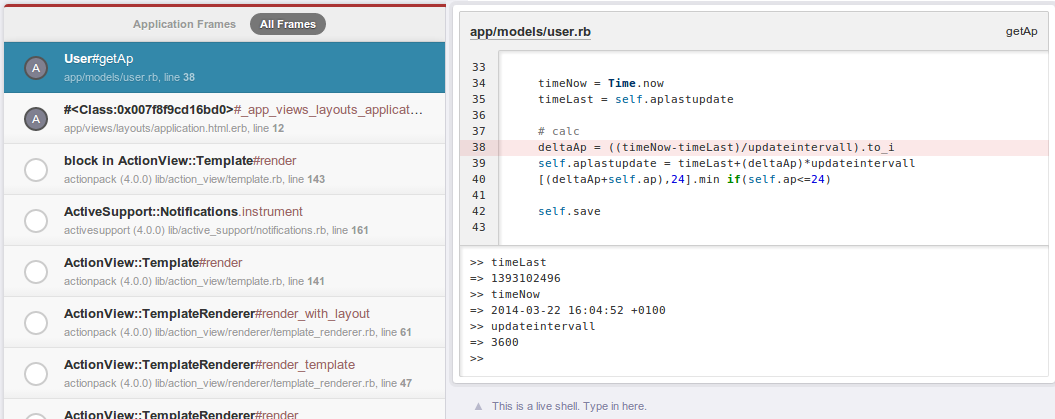
\includegraphics[width=155mm]{images/ch5_img08_livebinding.png}
\caption{Interaktives Debugging mit \glqq better\_errors\grqq{} und \glqq binding\_of\_caller'}
\label{img:ch5_img08_livebinding}
\end{center}
\end{figure}

Für die Entwicklung von Software ist es essentiell beliebig den Code wiederherstellen zu können und einfach neue Funktionen auszuprobieren. Diese Anforderung bedienen Software Systeme zur Versionsverwaltung. 
Die Auswahl wurde auf ein Open-Source System gelegt. Am weitesten verbreitet sind zur Zeit Subversion und Git. Letzteres bietet Möglichkeit einer nicht linearen Entwicklung \cite{Bird.2009}.
Die Wahl fiel speziell auf Subversion, da es im Gegenzug zu CVS das Versionsschema nicht auf einzelne Dateien sondern auf das ganze Projekt bezieht.
Das hat den Vorteil, dass das Hinzufügen einer neuen Funktion nicht in der Hauptklasse Version 50 und in der Methodenklasse Version 70 gespeichert wird, sondern in einer gemeinsamen Version.
Somit ist es für den Entwickler möglich den Zusammenhang zwischen den einzelnen Dateien direkt zu erkennen, da die neue Funktion z.\,B. in der Revision 60 in beiden Dateien erkennbar ist.
Die Verwendung von Git wurde in Erwägung gezogen, aber Aufgrund der Tatsache, dass das Projekt nur einen Entwickler besitzt, wurde dies als unproblematisch angesehen. Ein späterer Transfer in ein Git-Projekt ist problemlos mit \glqq git-svn clone\grqq{} und weiteren Anpassungen möglich. Der Transfer ist in jedem Fall zu empfehlen, gerade wenn das Framework später mit mehreren Entwicklern weiterentwickelt wird.

\section{Implementierung des Geogameframeworks}
\label{ch5:s:Implementierung}

\subsection*{Realisierung}

Nachdem alle Anforderungen, Schnittstellen und Werkzeuge des Frameworks festgelegt wurden, konnte mit der Umsetzung begonnen werden.
Wie bereits in Kapitel XX beschrieben lässt sich das Framework in drei Module unterteilen auf die im nachfolgenden jeweils entsprechend eingegangen werden soll.

\begin{itemize}

\item GameAPI (Overpass API)
\item Beispiel Spiel
\item Evaluationstool

\end{itemize}

\subsubsection*{GameAPI}

Die GameAPI stellt die API des GameFrameworks dar. Sie wird dazu verwendet um die Spielfelder entsprechend aufzubauen.
Generell gibt es X unterschiedliche Funktionen die zur Verfügung gestellt werden.
Es wird unterschieden zwischen den Locations (im Beispiel Spiel Flaggen) sowie den lokalen Händlern.
Der Aufruf der Schnittstelle erfolgt mittels eines RestFULL Request mit folgenden Parametern:
\\\\
\url{SITE\_URL/overpass\_api/getLocation.json?s=49&w=10&n=50&e=11&tag=highway=bus\_stop}
\\\\
Der Aufruf kann sowohl als GET als auch als POST Request durchgeführt werden. Die Parameter s,n,w,e sind essentiell und der Parameter tag ist optional.
Die Parameter sind zwei Werte. Die ersten vier Parameter beschreiben die angefragte Bounding Box ab. S steht hierbei für South (Bounding Box Minimum Latitude), N für North (Bounding Box Maximum Latitude), W für West (Bounding Box Minimum Longitude) und E für East (Bounding Box maximum Longitude). Der Letzte Parameter tag beschreibt den zu verwendenden OSM Tag. Wird der entsprechende Tag nicht angegeben so wird der im Framework hinterlegte Default tag verwendet. Ziel ist es hierbei den Standard Wert für das darauf aufbauende Beispiel Spiel zu verwenden und den optionalen Parameter tag für die Evaluation einzelner Tags -- konkret der jeweiligen key-value-Paare zu ermöglichen. Nachdem der entsprechende Aufruf erfolgt ist. Wird das Ergebnis als GeoJSON mit entsprechender Properties zurückgeliefert.
\\\\ %% settings for current code
\lstset{
   language=JavaScript,
   backgroundcolor=\color{white},
   extendedchars=true,
   basicstyle=\scriptsize\ttfamily,
   showstringspaces=false,
   showspaces=false,
   frame=single,
   numbers=left,
   numberstyle=\scriptsize,
   numbersep=9pt,
   tabsize=2,
   breaklines=true,
   showtabs=false,
   captionpos=b
}

\begin{lstlisting}[caption=GeoJSON Response Location (Reduziert), label=code:ch5:geojson01]
{
  "type": "FeatureCollection",
  "features": [
    {
      "type": "Feature",
      "geometry": {
        "type": "Point",
        "coordinates": [
          10.8748794,
          49.9002723
        ]
      },
      "properties": {
        "popupContent": "Test",
        "id": "301967628",
        "user_id": "neutral",
        "prestige": 0
      }
    }
  ]
}
\end{lstlisting}

Wie in Code \ref{code:ch5:geojson01} zu sehen ist die Antwort der API analog zur GeoJSON Spezifikation \cite{Butler.2008}.
In jedem Fall enthält ein GeoJSON ein Objekt. Enthält das GeoJSON mehr als ein Objekt so sind diese in einer FeatureCollection gesammelt. Diese wiederum enhält entsprechende Objekte.
Jedes Objekt nimmt einen der nachfolgenden Objekttypen an:
 \glqq Point\grqq, \glqq MultiPoint\grqq, \glqq LineString\grqq, \glqq MultiLineString\grqq, \glqq Polygon\grqq, \glqq MultiPolygon\grqq{} oder \glqq FeatureCollection\grqq. Für die Implementierung des Frameworks wird allerdings nur Point und FeatureCollection genutzt. Reduzierung auf Points ist der Tatsache geschuldet, dass durch die Transformation in Virtuelel Nodes lediglich feste einzelne Spielelemente existieren die auf einen Punkt reduziert wurden. Daher ist das passendste Element im GeoJSON ebenfalls der Point. Neben den Koordinaten des Punktes können zusätzlich weitere Attribute frei definiert werden. Diese für das Gameframework unter anderem id, user\_id und prestige. Ersteres beschreibt die virtuelle Node Id des OSM Objekte von dem das Node abstammt. In diesem Fall lässt sich anhand der Zahl erkenne, dass es sich um ein Node handelt und kein Way oder Relation von dem der Punkt abstammt. Das Attribut user\_id beschreibt den Besitzer des Eleements. Für das Beispiel Spiel wurde hier keie konkreten Ids sondern die Stati \glqq neutral\grqq,\glqq owner\grqq,\glqq foe\grqq{} bestimmt. Mit einer einfachen Anpassung einer Zeile im Framework können hier auch direkt die Userid ausgegeben werden. Sofern die Schnittstelle ohne Session von extern aufgerufen wird, gibt es nur den Zustand \glqq neutral\grqq{} oder \glqq foe", da ein Anonymer Zugriff keinem eingeloggtem User zugeordnet wird. Ist hingegen ein User authentifiziert über das Beispiel Spiel so erhält er zusätzlich die Information ob die aktuelle Flagge in seinem Besitz ist.
Das Attribut Prestige gibt ganz normal den aktuelle n Prestige Wert der Flagge zurück. In diesem Fall handelt es sich um ein neutrales nicht bisher eingenommene Flagge die daher automatisch den Wert 0 hat und noch nicht in der Datenbank persistiert wurde. Eine Aussgae ob ein Objekt entsprechend persistiert wurde oder nicht kann derjenige der die API verwendet nicht erkennen. Dies ist aber auch nicht notwendig, da 
die Persistierung transparent\footnote{im englischen Sinne} vor dem Spieler und gegenüber dem Schnittstellenbenutzer ist.

Die nächste Schnittstelle stellt die Händlerschnittstelle dar. Über diese können die Händler in einer vorgegebenen Bounding Box abgefragt werden, analog zu den Flaggen.
\\\\
\url{SITE\_URL/vendors/getVendors.json?s=49&w=10&n=50&e=11}
\\\\
Im Gegensatz zu einem Spielelement enthält das GeoJSON des Händlers allerdings weniger Attribute, wie in Codebeispiel \ref{code:ch5:geojson02} zu sehen.
\\\\
\begin{lstlisting}[caption=GeoJSON Response Vendor (Reduziert), label=code:ch5:geojson02]
{
        "type": "Feature",
        "geometry": {
            "type": "Point",
            "coordinates": [10.869845151901245, 49.902191491264695]
        },
        "properties": {
            "popupContent": "Insel 11"
        },
        "id": 2
    }
\end{lstlisting}

Die Standardattribute sind gleich, jedoch wurden die Properties reduziert. \glqq popupContent\grqq{} beschreibt den Inhalt des Popup-Fensters. In diesem Fall werden hier die Namen der Händler ausgegeben. Darüber hinaus hat auch jeder Händler eine Id. Diese sind jedoch nicht an OSM Elemente gebunden sondern für das Framework spezifisch.

\subsubsection*{Beispiel Spiel}

Das Beispiel Spiel stellt eine Proof of Concept Implementierung dar, welche auf dem Gameframework aufbaut. Es dient vor allem zum Test des Frameworks und kann später ausgebaut oder ersetzt werden. Das Beispiel Spiel lässt sich in drei Bereiche aufteilen. Zunächst wurde das Spielfeld mittels Leaflet implementiert.

\begin{figure}[H]
\begin{center}
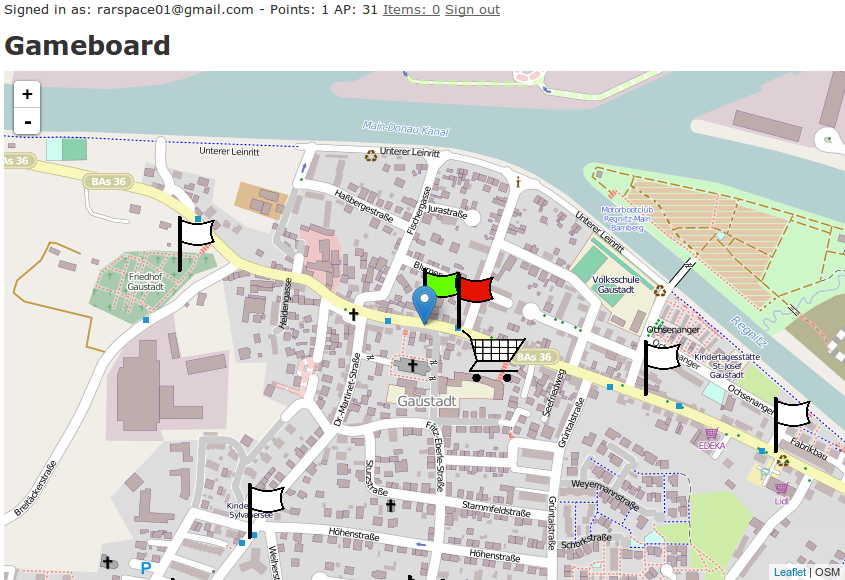
\includegraphics[width=150mm]{images/ch5_img09_gameboard.png}
\caption{Grundansicht -- Spielfeld}
\label{img:ch5_img09_gameboard}
\end{center}
\end{figure}

Das Spielfeld ist in Abbildung \ref{img:ch5_img09_gameboard} zu sehen. In der initialen Sicht wird das Spielfeld mittels HTML5 Geo Api auf die aktuelle Position zentriert. Die Karte selbst zeigt die Standard OSM Tiles. Diese können beliebig ersetzt werden. Gerade in Innenstädten kann es Sinn machen, entsprechend ein anderes Rendering zu verwenden. Eine Übersicht der kostenlosen Tileserver ist unter \url{http://wiki.OpenStreetMap.org/wiki/Tiles} zu finden. Möchte man über diese hinaus andere Styles verwenden und nicht selbst ein entsprechenden Tile-Renderingserver aufsetzten, so ist es zu empfehlen auf entsprechende Dienste wie z.\,B. MapBox\footnote{\url{https://www.mapbox.com/}} zurückzugreifen. Auf der Karte selbst sind per Layer die entsprechenden Spielelemente, sowie Händler eingebunden. Bewegt der Spieler den Kartenbereich oder bewegt er sich physikalisch fort, so werden die Daten entsprechend nachgeladen. Die Daten werden mittels GameAPI über das Framework ausgelesen und als GeoJSON eingebunden. Möchte nun der Spieler mit den entsprechenden Spielelementen interagieren, so muss er nur auf das entsprechende Element klicken. Im Beispiel Spiel öffnet sich dann je nach Elementtyp entweder die Übersicht der jeweiligen Flagge oder aber der Händler. Durch die Interaktion kann sich der Spiele über den aktuellen Prestige-Stnd informieren, sowie die Flagge angreifen. Dies kann der Spieler allerdings nur, wenn er sich im Umkreis von 40 Metern zur Flagge befindet. Beim AJAX Request, welcher der Spieler bei einem Angriff entsprechend durchführt, wird dieses sichergestellt. Der Aktionradius von 40 Meter soll sicherstellen, dass auch bei einer höheren GPS-Ungenaugikeit der Spieler trotzdem mit der Umgebung interagieren kann.
Beim Händler erhält der Spieler eine Übersicht über die verfügbaren Items. Im Gegensatz zu den Flaggen werden die Informationen über die jeweiligen Händler nicht direkt bei dem Abruf aller Händler mitgeteilt, sondern explizit für den jeweiligen Händler angefordert. Somit wird sichergestellt, dass die Synchronisierung möglichst zeitnah ist und der Spieler eine aktuelle Übersicht über das Inventars des virtuellen Händlers erhält.

Den aktuellen Punktestand kann der Spieler von der oberen Statusleiste entnehmen. Dieser berechnet sich anhand aller Flaggen die der Spieler eingesammelt hat. Dank Active Record in Verbindung mit Rails kann die Abfrage stark vereinfacht werden werden:
\\
\lstset{
   language=Ruby
}

\begin{lstlisting}[caption=Ruby - Abfrage der Spielerpunkte, label=code:ch5:activerecord01]
points = Flag.sum(:prestige, :conditions => ['user_id = ?',self.id])
\end{lstlisting}

Direkt daneben ist die Anzeige für die verbliebenen Aktionspunkte. Diese werden alle 60min um eins erhöht bis diese 24 Aktionspunkte erreichen. Der letzte Punkt stellt die Item-Übersicht dar. Über diese kann der Spieler seine aktuellen Items sich anzeigen lassen und je nach Bedarf diese auch entsprechend verwenden. Die Items werden erst mit dem klick auf das Inventar explizit per AJAX nachgeladen. zuvor kann der Spieler jedoch die Anzahl seiner Items in der Statusleiste sehen.
\\\\
Im Gegenzug dazu gibt es die Oberfläche für die Pflege der einzelnen Händler. Hierfür werden als Basis, durch Scaffolding generierte Formulare verwendet. Diese wurden entsprechend um zusätzliche Funktionen wie einem Leaflet map picker, sowie der dazugehörige JavaScript Code ergänzt. Zunächst kann der Spielleiter sich eine Übersicht der Händler über die nachfolgende Url aufrufen:
\\\\
\url{SITE\_URL/vendors}
\\\\
In der Übersicht kann er bestehende Händler direkt löschen, Neue anlegen oder Bestehende bearbeiten. 
Legt der Spielleiter einen Händler an, so wird ihm nicht nur eine Liste an Attributen angezeigt, sondern er erhält auch eine Leaflet Karte, die entsprechend auf der aktuellen Position zentriert ist. Über diese kann er frei auf der Karte einen Marker für die Position des Händlers setzen. Intern werden die Koordinaten des Markers entsprechend gespeichert und in der Datenbank hinterlegt. Möchte der Spielleiter nun einen der Händler bearbeitne wird analog dazu das FOrmular wieder aufgerufen und entsprechend mit den Daten aus der Datenbank gefüllt. Gleiches gilt auch für die Leaflet Karte auf der der zuvor gespeicherte Marker hinterlegt wurde. In diesem Mdus hat der Spielleiter zudem die Möglichkeit Items direkt dem Händler zuzuweisen die dann später zum Verkauf stehen. Für die Einfachheit werden entsprchend alle freien noch nich zugewiesenen Items entsprechend angezeigt und können mit einem einfachen Klick hinzugefügt werden. Hierfür sind entsprechende Controller für die Händler Klasse erstellt worden, die das Kaufen und Zuweisen von Items ermöglichen.

Über die nachfolgende Unterseite, findet die Pflege der Items statt:
\\\\
\url{SITE\_URL/items}
\\\\
Auf dieser Seite erstellt der Spielleiter alle Items die den Händlern zur Verfügung stehen sollen. Hierbei handelt es sich ebenfalls um ein nach typischen Scaffolding erzeugtem Formularmuster zur Pflege der einzelnen Daten. Jedes Item ist dabei explizit als Objekt angelegt und kann einem Itemtyp angehören. Eine Anpassung der Items ist nach der Erstellung möglich. Im Zuge des Beispiel Spiels wurde auf eine umfangreiche Rollen und Rechtevergabe verzichtet, da der Fokus auf den Spielelemente lag. Nichtsdestotrotz können diese entsprechend erweitert werden, je nachdem für welches Spiel das Framework eingesetzt werden soll.

\subsubsection*{Evaluationstool}

Das Evalutationstool verwendet die zuvor in der GameAPI beschriebene Schnittstelle um Spielfelder zu bewerten bzw. zu evaluieren. Hierfür wird die zusätzliche Möglichkeit genutzt konkrete tags zu einer Bounding Box abzufragen. Für eine Evaluation verwendet das Tool eine vorgegebene Liste an Key-Value Paaren und eine Geo-Koordinate, die zu einer Bounding Box erweitert wird. Basierend auf dem im Kapitel \ref{ch:CH6_qualtiy_of_gameboards} beschriebenen Ansätzen werden die einzelnen Spielfelder jeweils Evaluiert. Für die Evaluation der Spielfelder müssen die Entfernung zwischen den einzelnen Punkten berechnet werden. Hierbei werden nicht die euklidische Distanz zwischen den Geo-Koordinaten berechnet sondern es muss die reale Netzwerkdistanz auf dem Straßennetz berechnet werden. Da der Spieler nicht nur per Auto sondern bevorzugt auch per Fahrrad und im besten Fall zu Fuß das Spiel nutzt, ist ein Fußgängerrouting notwendig. Das bedeutet Wege die nur für Fußgänger zugänglich sind, müssen ebenfalls beachtet werden. Da OpenStreetMap im Vergleich zu Google Maps im Hinblick auf den Datenumfang an dieser Stelle einen Vorteil hat, ist es sinnvoll hierfür auf OSM zurückzugreifen. Durch den Umfang und Anzahl der Abfragen die sich durch die Evaluationsmethoden ergeben, ist es sinnvoll die Anfragen nicht an einen Onlinedienst zu stellen sondern diese offline mit einem dedizierten Routing durchzuführen. Für das offline Routing mit OSM gibt es diverse Bibliotheken, aufgrund der Anforderung möglichst viele Abfragen zeitnah durchzuführen wurde sich für das Tool GraphHopper entschieden. Dieses bietet ein vollständiges Offline Routing auf Basis von OSM Rohdaten \cite{Karich.2014}. Hierfür erstellt GraphHopper zunächst entsprechende Indexdateien auf denen dann später das Routing stattfindet. Diese enthalten in binärer Form die agregierten Pfade des Netzwerkes.

Mit Hilfe von GraphHopper ist es nun Möglich entsprechend schnelle Abfragen durchzuführen. Da die GraphHopper Bibliothek selbst nicht für Parallelisierung ausgelegt ist, wurde das Evaluationstool entsprechend optimiert um die Ressourcen eines Rechners/Servers vollständig auszunutzen. Dadurch kann die Laufzeit bei mehreren Tags je nach Anzahl der vorhandenen CPUs auf $\frac{1}{lc}$ verkürzt werden. Wobei lc die Anzahl der logischen CPUs darstellt. Bei einer Laufzeit von $\mathcal O(n^2)$ ist dies unerlässlich.
Da GraphHopper in Java realisiert wurde, wurde das Evaluationstool analog dazu ebenfalls in Java entwickelt.

\subsection*{Tests}

Da das Framework später entsprechend für verschiedene Spiele genutzt werden soll, muss dieses entsprechend getestet werden.
Hierbei wird unterschieden zwischen Low-Level-Tests und High-Level-Tests\cite{Pol.2002},
Unter Low-Level-Tests sind solche Test zu verstehen, die während der Implementierung an Teilen des Systems stattfinden. Bei High-Level-Tests wird das komplette System getestet. Einer der Low-Level-Tests ist der Modultest. Bei diesem werden einzelne Module im Programm getestet.  

Für das Gameframework wurden die einzelnen Module unabhängig voneinander getestet. Zunächst wurden speziell die Schnittstellen zu OSM und Overpass getestet. Hierbei wurde vor allem kontrolliert, dass die Übergabeparameter, sowie das Datenformat korrekt ist und die Interpretation der Daten korrekt vorgenommen wird.
Nachdem die die GameAPI mit ihrer Transformation der OSM Elemenete in Spielelemente implementiert wurde, ist das Beispiel Spiel entsprechend darauf aufgebaut worden. Hierzu wurde die korrekte Transformation der Elemente anhand von speziellen Tags manuell überprüft. Hierzu wurde \url{http://taginfo.OpenStreetMap.org} verwendet. Dies Seite bietet einen statistischen Überblick aller tags in OSM sowie die Verteilung auf die Elemente Relation, Way und Nodes. Der Test erfolge anhand von Key-Value Paaren die jeweils explizit nur als einer der drei Typen bevorzugt gemappt werden.

Das Spiel selbst musste ebenfalls getestet werden. Da ein ortsbezogenes Spiel als Grundlage die Position de Spielers verwendet und ein Debugging unterwegs sich als schwierig gestaltet, ist es am besten die GPS-Koordinate zu simulieren. Hierfür gibt es entsprechende Plugins für die am weitesten verbreiteten Browser, wie Chrome oder Firefox. mit Hilfe von diesen kann die Position welche die HTML5  Geo API zurückliefert entsprechend verändert werden. Darüber hinaus ist es auch möglich die Genauigkeit der GPS Position, sowie das Bewegungs-Event zu triggern. Mit Hilfe von diesem können alle ortbezogenen Funktionen des Beispiel Spiels auch dirke twährend der Entwicklung getestet werden.
Für die Nutzung des Spieles auf Smartphones eignet sich darüberhinaus der Einsatz von entsprechenden Emulatoren. Für Android und FirefoxOS sind diese frei verfügbar. Für iOS fallen jährliche Gebühren an und der Emulator inkl. SDK ist nur unter der neusten Mac OS X Version verfügbar.

Tests für das Evaluationstool wurden vorwiegend für die Performance und den Werten durchgeführt.
Konkrete Unit-Tests wurden für das Framework aus Zeitgründen nicht entwickelt, sollten aber als nächster wichtiger Punkt entsprechend implementiert werden.

Als High-Level bzw. Blackbox Test wurden die in den Usecase Diagramm beschriebenen Anwendungsfälle getestet. D.h. die Funktionen die den jeweiligen Akteuren zur Verfügung stehen wurden ohne Betrachtung.

\subsection*{Probleme}

Während der Umsetzung sind auf einige Besonderheiten gestoßen, welche eine spezielle Anpassung oder Überlegung erfordert haben. Im nachfolgenden soll kurz auf diese eingegangen werden um die Erkenntnisse festzuhalten. Idealerweise können diese in zukünftigen Untersuchungen und Implementierungen entsprechend vermieden bzw. umgangen werden.

Ein erster Aspekt der von Relevanz, ist die Spezifikation der GeoJSON. Standardmäßig werden Koordinaten in der Reihenfolge Latitude, Longitude angegeben \cite{Schoeneberger.2002,Barzegar.1996,Maling.1991,}. Die GeoJSON Spezifikation hingegen sieht im Kontrast zum de facto Standard vor, dass zuerst die Longitude und dann die Latitude genannt wird \cite{Butler.2008}. Ist dies nicht bekannt, kann dies zu einigem Aufwand führen, der vermeiden werden kann.

Ein weiteres Problematik die im Zuge des Transformationsprozesses der Relations und Ways zu virtuellen Nodes mit einer mit Bitmasken codierten Eigenschaft, führte dazu, dass im Zuge der Verwendung mit Javascript Probleme auftraten. Dies äußerte sich darin, dass die Ids nach der Interpreation plötzlich auf unerklärlicher weise veränderte Werte annahmen. So kamen Abweichungen von bis zu 100 zu Stande. Nach längeren Debug Aufwänden wurde herausgefunden, dass die implizite Typisierung in JavaScript den Ganzzahlenwert der Id intern als Gleitkommazahl transferiert und dadurch unbewussterweise die 51Bit überschreitet nach denen die Mantisse der Gleitkommazahl beginnt. Durch diese Verschiebung wurden die hinteren Bits beim auslesen des long Wertes vernachlässigt. Um dieses Problem zu umgehen gibt es zwei Möglichkeiten. Entweder man teilt die Zahl auf Basis des 64bit long Wertes in zwei 32bit Integer Werte und legt diese in zwei Zahlen in JS ab. Sollten keine arithmetischen Operationen auf der Id durchgeführt werden sollen im JavaScript Code, dann empfiehlt es sich die Id explizit als String auszugeben, damit JavaScript diese nicht als Zahl interpretiert und versucht entsprechend umzuwandeln.

Ein weiterer Punkt stellt Turbolinks dar. Turbolinks ist ein Gem, welches Standardmäßig in Rails aktiv ist. Es sorgt dafür, dass bei einer Interaktion mit der Seite nicht die komplette Seite neu geladen wird, sondern nur die Teile des Html Codes, welcher sich geändert hat \cite{Gamble.2013}. Die Problematik die damit einhergeht sind Ajax Requests, welche über normale href links angestoßen werden. Eine typische Verwendung ist z.\,B.:
\lstset{
   language=Html
}

\begin{lstlisting}[caption=a href HTML Code, label=code:ch5:html01]
<a href='#\grqq{} onClick="saveItem(1);">Save</a>
\end{lstlisting}

Allerdings für der Klick auf \glqq Save\grqq{} in diesem Fall zu einem Neuladen der Seite durch Turbolinks. Befindet sich an dieser Stelle aber ein Javascriptcode mit Ajax request, passiert es, dass die Seite neu geladen wird anstatt den Code auszuführen, welcher z.\,B. eine Aktualisierung einer Zahl auf der Seite zur Folge hätte.
Um diese zu vermeiden muss Turbolinks explizit angewiesen werden, bei a href Links nicht aktiv zu werden. Dies kann man pro Link individuell setzten:

\begin{lstlisting}[caption=a href HTML Code - Turbolinks deaktiviert, label=code:ch5:html01]
<a href='#\grqq{} data-no-turbolink onClick="saveItem(1);">Save</a>
\end{lstlisting}

Dadurch wird sichergestellt, dass der entsprechende JavaScript Code ausgeführt wird und nicht einfach die Seite neugeladen wird.

Ein letzter Punkt, der zu Problemen führen kann ist der \glqq Zurück"-Button im Browser.
Durch diesen wird die vorherige Seite wieder aufgerufen, allerdings deren Javascriptcode nicht nocheinmal 1:1 getriggert wie beim laden der Seite. D.h. diverse Event-Listener welche auf \glqq OnDocumentReady\grqq{} z.\,B. mittels JQuery warten, werden nicht noch einmal aufgerufen. Wird dies nicht entsprechend in der Entwicklung berücksichtigt, kann es dazu führen, dass die Seite sich in einem nicht definierten Zustand befindet.

\newpage
\chapter{Evaluierung}
\label{ch:S6_Evaluierung}

\section{Qualität der Lösung}
\label{ch:CH6_qualtiy_of_solution}

Für eine Evaluation der in Kapitel \ref{ch:S4_Lösungsansatz} und \ref{ch:S5_Umsetzung} vorgestellten Lösung muss zunächst die Evaluationsmethode definiert werden. Für die Evaluation soll die Lösung der Arbeit mit der Problemstellung in Kapitel \ref{ch2:Problemstellunug} gegenübergestellt werden. Es wird untersucht inwiefern das Framework und das Beispiel Spiel zu einer Lösung der Problemstellung beitragen. Das Ergebnis der Evaluation soll entsprechend weitere Handlungsempfehlungen bzw. Verbesserungsvorschläge aufzeigen, sofern diese aufgrund der Evaluation notwendig sein sollten. 
Die vorgestellte Lösung soll im Hinblick auf die vier Hauptaspekte untersucht werden:

\begin{itemize}

\item Gamification unter Einbezug der Händler
\item Pervasive Games
\item Relokalisierbarkeit
\item Verwendbarkeit von OSM Daten

\end{itemize}

Die Evaluation der durch das Framework erzeugten Spielfelder und somit eine Bewertung der Relokalisierbarkeit wird in Kapitel \ref{ch:CH6_qualtiy_of_gameboards} behandelt.


\subsection*{Gamification}

Im Bezug auf die in Kapitel \ref{ch1:Einleitung} aufgestellte Motivation, soll die Lösung mittels Gamification den regionalen Händlern zu neuen Kunden führen können und bestehende entsprechend halten. Ziel ist es nicht zu überprüfen, ob und wie hoch der entsprechende Neukunden und Bestandskundenanteil durch die Lösung beeinflusst wird, sondern inwiefern entsprechende Elemente aus der Literatur umgesetzt wurden. Diese wiederum sollen die Möglichkeit für einen besseren Umsatz der Händler bieten.
In der Literatur wurden zunächst die rudimentären Elemente eines Gamification Prozesses herauskristallisiert. Für die softwaretechnische Umsetzung wurden bei der Implementierung die Anforderungen entsprechend umgesetzt, damit die Gamification-Elemente Points, Badges und Leaderboards problemlos verwendet werden können. Zudem wurden die Aspekte der klassischen Spieltheorie aufgegriffen und dadurch die Gamificationen Ansätze erweitert. Es wurden mehrere Optionen aufgezeigt, welche in Spielen umgesetzt werden können. Darüber hinaus wurden diese Aspekte mit entsprechenden Technologien wie NFC oder Bluetooth Low Energy in Verbindung gebracht, wie eine Integration der Spielelemente vor Ort bei den Händlern gestaltet werden könnte. Das Framework und das Beispiel Spiel bilden diese nicht alle ab, sind aber problemlos in der Funktionalität erweiterbar.
Durch die Kombination der Gamification Elemente und der Generierung von Spielelementen auf Basis der Umgebung in Kombination der lokale Händler wird das Maß der Immersion für die Spieler erhöht und der Effekt der Gamification verstärkt.
Für den Aspekt der Gamification lässt sich daher abschließend festhalten, dass die aufgezeigte Lösung einen Beitrag zur Lösung der Problematik der Gamification von Neukundenbesuchen bei regionalen Händlern liefern kann.

\subsection*{Pervasive Games  -- Anforderungen an ein Gameframework}

Im Zuge der Erstellung eines Frameworks zum Staging von Pervasive Games müssen mehrere Aspekte behandelt werden. Zunächst muss definiert werden, welche Grenzen des Magic Circle überschritten werden. Im Zuge dieser Arbeit lag der Fokus auf der Dimension Ort und Zeit. Das bedeutet, dass ein entsprechendes Spiel soll sowohl ortsunabhängig als auch zeitunabhängig gespielt werden kann. Die Ortsunabhängigkeit der vorgestellten Lösung wird durch die Relokalisierung mit Hilfe von OSM-Daten sichergestellt. Die zeitliche Unabhängigkeit ist dadurch sichergestellt, dass jeder Spieler sich individuell am Beispiel Spiel anmelden kann und es keine fest definierten Uhrzeiten oder Termine gibt um das Spiel zu spielen. Im Vergleich zu typischen Geogames ist es daher möglich auch über feste Uhrzeiten und Geografische Gebiete hinaus das Spiel zu spielen. Durch die entsprechende Formulierung der Anforderungen in Kapitel \ref{ch2:Problemstellunug} und \ref{ch4:s:Lösungen} und der Ausrichtung des Frameworks an diesen wurde sichergestellt, dass das Framework diese Anforderungen erfüllt. Da es sich in der Problemstellung um ein Echtzeitspiel handelt muss auch entsprechend im Framework sichergestellt werden, dass die Interaktion mit dem Spiel in Echtzeit erfolgen kann.
Durch die Modularisierung und Auskopplung der Evaluation der OSM Tags, ist es möglich die zeitintensiven Bewertung der Spielfelder unabhängig von der Spielfeldgenerierung durchzuführen. Dadurch ist wird es möglich, lediglich die relativ einfachen Prozesse zur Transformation der OSM-Elemente während der Laufzeit durchzuführen. Vergleicht man die durchschnittliche Antwortzeit des Frameworks, so ist diese ausreichend niedrig. Die Varianz ist wie in Abbildung \ref{img:ch6_img01_response_time} erkenntlich zu vernachlässigen.  Die Antwortzeit ist  abhängig von der Anzahl der OSM-Elemente in der Bounding Box und der Antwortzeit des Overpass API Servers, jedoch steigt diese nicht weiter, wenn die empfohlene maximale Anzahl an Spielelementen nicht überschritten wird. Die Evaluationsfunktion hingegen liegt bei 2-3 Minuten für ein Tag mit ca. 200 Elementen. Für ein Feld mit 1200 Elementen liegt diese bereits bei über 30 Minuten.

\begin{figure}[H]
\begin{center}
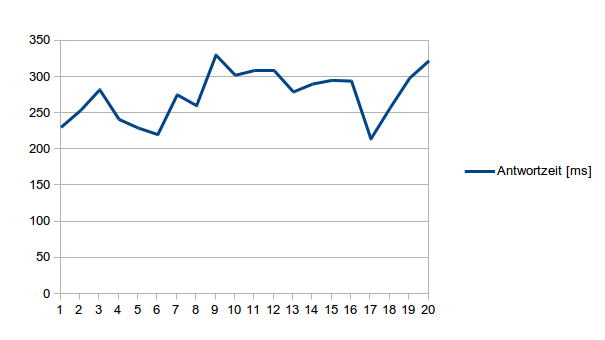
\includegraphics[width=150mm]{images/ch6_img01_response_time.png}
\caption{Antwortzeit der GameAPI für den Tag public\_transport = stop\_area}
\label{img:ch6_img01_response_time}
\end{center}
\end{figure}

Abweichungen der Antwortzeit sind weniger bedeutend, da das Spielfeld sich bereits vorher für den Spieler aufbaut und die Spielelemente mittels Ajax Request geladen werden. Darüber hinaus wird durch die dynamische Erweiterung der Bounding Box sichergestellt, dass alle Elemente am Rand der Karte bereits geladen sind. Das Nachladen der Elemente beim Fortbewegen kann daher auch minimal länger dauern, da das Spielfeld immer zentriert auf den Spieler ist.

Durch die Kapselung der einzelnen Module wird auch sichergestellt, dass eine Erweiterbarkeit der Spielmechanik ohne größeren Aufwand möglich ist. Das entsprechende Beispiel Spiel kann problemlos erweitert werden oder aber durch ein beliebiges anderes Spiel ersetzt werden.
Hierbei zeigt sich, dass die Anforderung für die Flexibilität des Frameworks hinsichtlich seiner Erweiterbarkeit und Austauschbarkeit gegeben ist.

\subsection*{Relokalisierbarkeit}

Der nächste essentielle Aspekt der Problemstellung war die Relokalisierbarkeit. Ziel war es im Zuge des zu vereinfachenden Stagings dem Spielleiter entsprechend eine Möglichkeit an die Hand zu geben, welche im auch ein Spielen außerhalb eines festen Bereiches ermöglicht. Hierzu wurden entsprechende OSM-Daten verwendet die durch eine Transformation zu Spielelementen umgewandelt wurden. Durch die entsprechende Evaluation der OSM-Tags im Voraus wird sichergestellt, dass der jeweils beste Tag für die getesteten Umgebungen ausgewählt wurde.
Die Transformation der OSM-Elemente funktioniert problemlos, speziell auch mit Relationen und Ways, wie in Abbildung \ref{img:ch6_img02_transform} zu erkennen ist. Auf der linken Seite sind die Daten aus OSM respektive Overpass zu sehen. Auf der rechten Seite sind hingegen die vom Framework erzeugen Spielelemente ersichtlich.


\begin{figure}[H]
\begin{center}
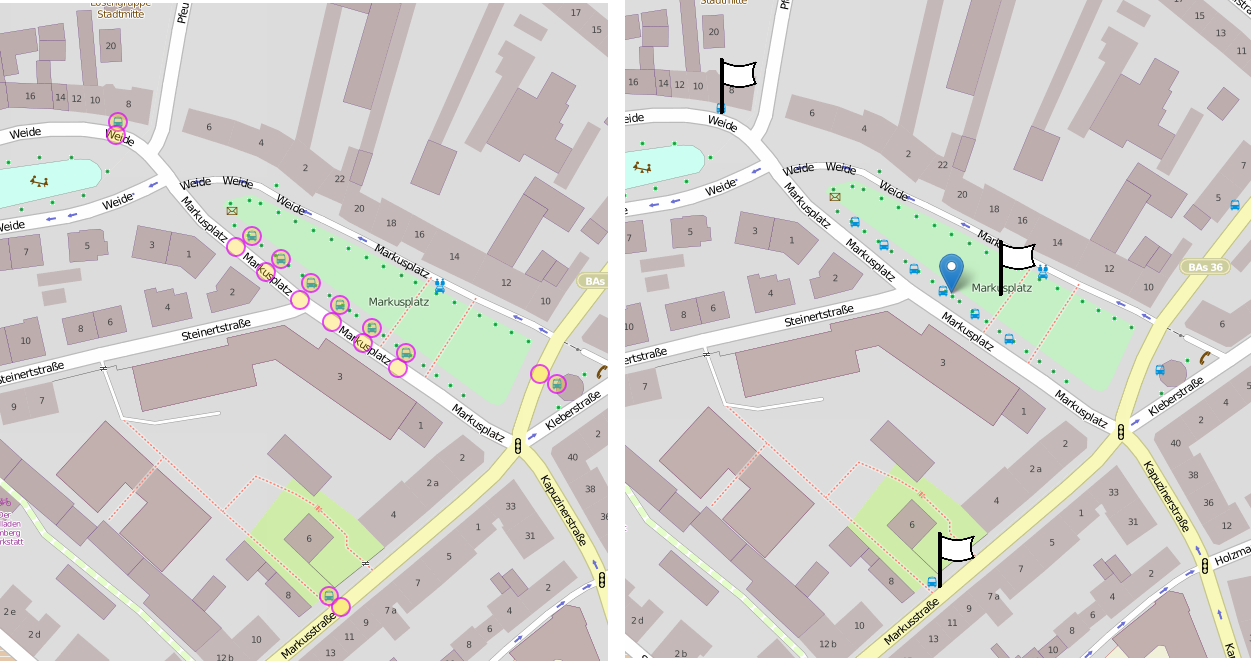
\includegraphics[width=150mm]{images/ch6_img02_transform.png}
\caption{OSM-Daten im Vergleich zu den transformierten Spielelementen}
\label{img:ch6_img02_transform}
\end{center}
\end{figure}

Sofern eine entsprechende Evaluierung im Voraus sichergestellt wurde, sind die Spielfelder ohne Einschränkungen nutzbar.
Einen Nachteil der Fokussierung auf ein einzelnes Key-Value Paar in OSM, ist die Möglichkeit, dass es z.\,B. in Regionen in denen eine geringere Mapping Qualität vorliegt, im Extremfall keine Spielelemente zur Verfügung stehen könnten. Diese Problematik könnte in diesem Fall durch eine einfache Anpassung des Frameworks gelöst werden. Hierzu müsste intern eine Liste mit alternativen Tags vorgehalten werden. Diese Liste könnte dynamisch auf Basis von \url{http://taginfo.openstreetmap.org/tags} gefüllt werden. Beim Aufruf der GameAPI müsste das Framework nur die vorhandene Zahl der Spielelemente prüfen und bei einer Unterschreitung eines vordefinierten Wertes automatisch den nächsten alternativen Tag verwenden. Zwar führt dies dazu, dass potentiell die Auswahl der Spielelemente für den Spieler schwerer nachvollziehbar ist, jedoch würde dies sicherstellen, dass auch im Worst Case Szenario entsprechend ausreichend Spielelemente generiert werden.

Somit lässt sich feststellen, dass die Relokalisierung problemlos funktioniert und auch entsprechend für den Einsatz mit Pervsaive Games geeignet ist. Ein offener Punkt ist eine weitere Optimierung für das Worst Case Szenario für den Fall, dass der optimale Tag im lokalen Bereich keine Spielfelder liefern kann.

\subsection*{Verwendbarkeit von OSM Daten}

Eine Fragestellung zu Beginn der Arbeit war die Verwendbarkeit von OSM-Daten im Zuge von Pervasive Games.
Die Anforderungen an die Daten im Vergleich zu einer Navigationssoftware sind beim Framework vergleichsweise gering.
Es muss eine korrekte Klassifikation stattfinden und die Abweichung der Position sollte vorzugsweise nicht mehr als der Aktionsradius des Spielers betragen. Dadurch wird erreicht, dass alle Spielelemente auch entsprechend von den Spielern physisch erreichbar sind.
Fehler bei der Klassifikation können vorkommen, da es immer der Fall sein kann, dass die Daten nicht entsprechend korrekt gemappt wurden.
Dies ist aber im Zusammenhang des Frameworks nicht weiter relevant, da deswegen maximal das entsprechende Element/Objekt nicht auf dem Spielfeld erscheinen wird. Durch das Fehlen wird aber die Funktionalität des jeweiligen Spieles selbst nicht beeinträchtigt. Hierdurch wird lediglich die Verteilung auf dem Spielfeld beeinflusst. Probleme mit dem Spielfeld bei zu wenig Elementen wurden bereits angesprochen und mögliche Lösungen aufgezeigt.
Die Transformation der OSM-Daten stellt sicher, dass auch Mapping Fehler, z.\,B. das rekursive Verweisen von Relations, keine Probleme entstehen. Es wird sichergestellt, dass in jedem Fall die Transformation stattfindet.
Abschließend ist festzuhalten, dass OSM ohne Einschränkungen nutzbar ist.
Gründe hierfür sind die Ergebnisse in der Literatur, welche OSM eine ausreichende Datenqualität zusprechen und OSM auch hinsichtlich der Lizenz für kommerzielle Produkte verwendbar ist. Darüber hinaus lieferten allen Tests mit dem Gameframework gute Ergebnisse. 

\subsection*{Abschließendes Ergebnis}

Für den Spielleiter lässt sich daher festhalten, dass die Anforderungen für ein einfaches Staging erfüllt werden. Darüber hinaus findet auch die geforderte Modularisierung der einzelne Funktionen statt. Die einzelnen Komponenten ermöglichen es mithilfe von OSM-Daten entsprechende Spielfelder zu erzeugen, welche unter Einbindung der virtuellen Händler und entsprechender Gamification Elemente des Beispiel Spiels zu einer Lösung der in Kapitel \ref{ch2:Problemstellunug} vorgestellten Probleme führt.


\section{Qualität der Spielfelder}
\label{ch:CH6_qualtiy_of_gameboards}

Ein wichtiger Aspekt für die Nutzung des Frameworks stellt die Qualität der Spielfelder dar.
Wie bereits angedeutet, wird für die Auswahl der Spielelemente das jeweilige OSM-Tag verwendet und auf Basis des Tags die OSM-Elemente zu Spielelementen transformiert. Um die jeweiligen Tags bewerten zu können muss daher eine Evaluations-Methode der Spielfelder definiert werden.
Das Ziel ist es somit durch den Vergleich mehrerer Lokalitäten den optimalen Tag für alle Spielfelder zu finden. Somit wird ein Tag gesucht, der möglichst an allen Standorten zu einem bestmöglichen Ergebnis führt.
Um die Qualität eines Spielfeldes beurteilen zu können muss zunächst näher definiert werden, welche Kriterien ein gutes Spielfeld ausmachen. 
Betrachtet man zunächst Punkte auf einer normalen zweidimensionalen Fläche so lassen sich nachfolgende Kriterien festlegen.
Zum einen muss sichergestellt werden, dass der Abstand aller Punkte gleich zu den anderen Nachbar-Punkten ist. Gleichzeitig muss vermieden werden, dass es zu einem Clustern der Punkte kommt. Ein ideales Feld für eine zweidimensionale Fläche ist in Abbildung \ref{img:ch6_img03_ideal2d} zu sehen.

\begin{figure}[H]
\begin{center}
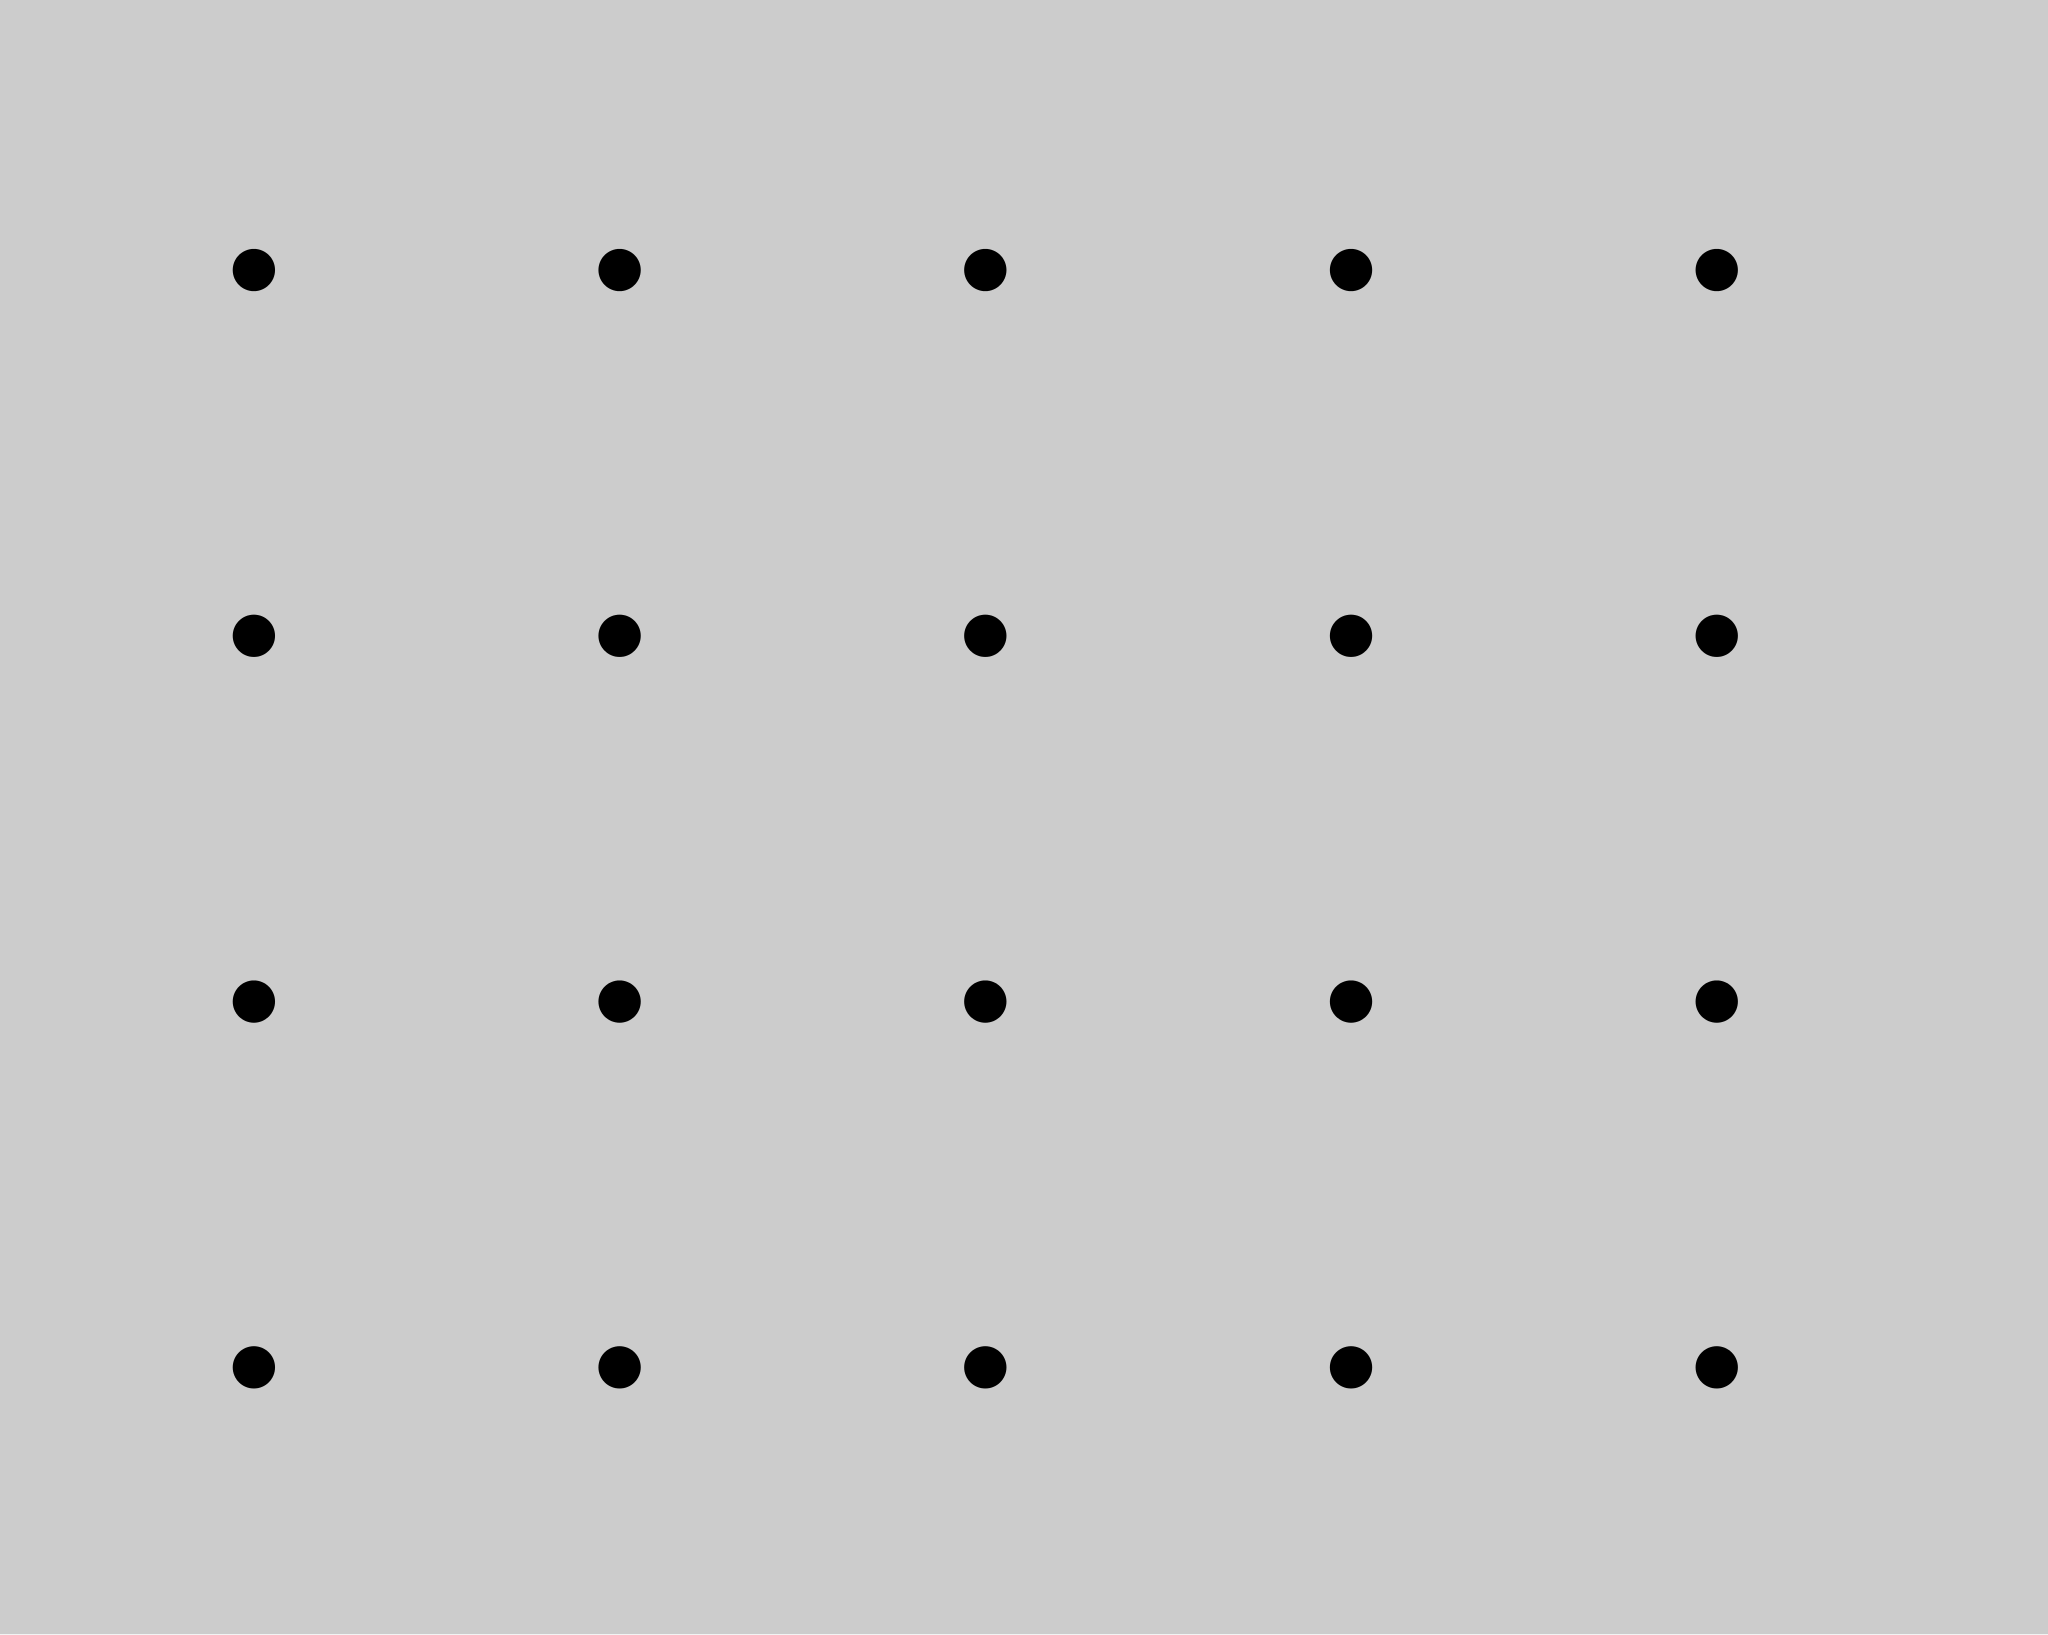
\includegraphics[width=100mm]{images/ch6_img03_ideal2d.png}
\caption{Ideale Verteilung von Elementen auf einer zweidimensionalen Fläche}
\label{img:ch6_img03_ideal2d}
\end{center}
\end{figure}

Für den Transfer der Kriterien auf den Anwendungsfall, muss berücksichtigt werden, dass die Spieler sich nicht per Luftlinie fortbewegen können. Diese können sich auf Grund der ortsbezogenen Affordanzen nur über die üblichen Wege fortbewegen. Diese Problematik betrifft auch die Fälle, in denen es geografische Hindernisse gibt. Beispielsweise wenn zwei Stadtteile zwar direkt nebeneinander liegen, diese aber durch einen Fluss getrennt sind. Diese Einschränkungen spiegeln sich alle im Wegnetz wieder. Daher muss untersucht werden, wie die optimale Verteilung der Spielelemente auf Basis der nächstgelegenen Wege stattfinden kann. Da die Punkte allerdings nicht selbst ausgewählt werden sondern aus OSM stammen und das Finden der besten Punkte ein zu komplexes Optimierungsproblem darstellen würde, muss ein anderer Ansatz verfolgt werden. Es ist somit notwendig die Abstände zwischen den einzelnen Spielelementen  zu bestimmen. Hierzu ist es notwendig die kürzeste Route zwischen zwei Punkten zu finden.
Da die meisten Routinglösungen reine Straßen bevorzugen, aber selten auch ausreichende Fußwege aufweisen, soll in diesem Fall wiederum auf OSM gesetzt werden.
Ziel soll es sein die Distanz zwischen den Spielelementen durch ein Offline Routing unter Verwendung von OSM zwischen den einzelnen Punkten zu bestimmen.
Zunächst muss aber bestimmt werden, welche der Spielelemente begutachtet werden. Hierfür werden dem entwickelten Evaluationstool jeweils ein OSM-Tag für die Auswahl der Spielelemente, sowie eine entsprechende Koordinate übergeben. Anhand dieser Information baut das Evaluationstool zwei Bounding Boxen. Diese werden unterschieden in die innere und äußere Bounding Box. Erstere enthält alle Punkte die untersucht werden sollen und letztere alle Punkte die zur Beurteilung herangezogen werden. Dieses Vorgehen ist nötigt, da ansonsten die Punkte an den Ecken der inneren Bounding Box bei einer Bewertung benachteiligt werden würden.
Die Anordnung der Bouding Boxen ist in Abbildung \ref{img:ch6_img04_bbox} zu sehen.
Die innere Bounding Box (schwarz) wurde im konkreten Fall auf 2,5km Breite und Länge 6,25km$^2$ festgesetzt. Im Gegensatz dazu steht die äußere Bounding Box (rot), welche um die innere um die maximale Evaluationsdistanz erweitert wurde. Im konkreten Fall soll diese Distanz 700 Meter darstellen, welches die Distanz von 10 Minuten Fußweg widerspiegelt. Die Wahl ist auf 10 Minuten gefallen um eine ausreichende Dichte der Spielfelder zu erreichen und die Spieler zudem zur Fortbewegung zu motivieren.


\begin{figure}[H]
\begin{center}
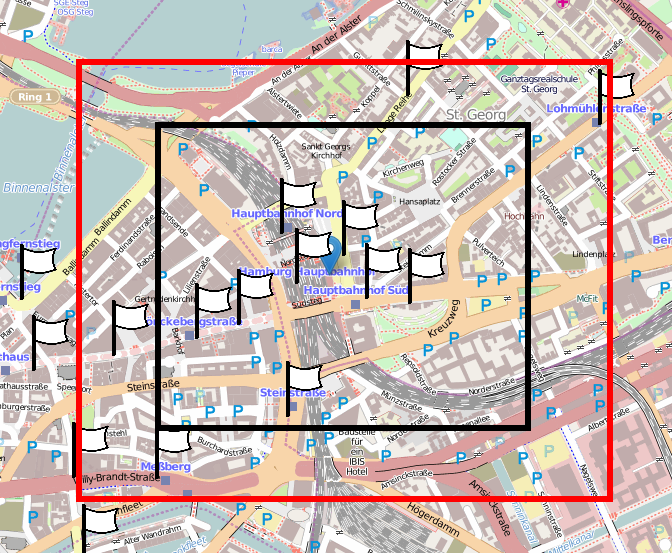
\includegraphics[width=100mm]{images/ch6_img04_bbox.png}
\caption{Inner und äußere Bounding Box zur Evaluation}
\label{img:ch6_img04_bbox}
\end{center}
\end{figure}

Zur Evaluation wurde eine Abwandlung der k-Nearest Neighbours Methode, konkret die count Nearest Neighbours gewählt.
Sie basiert auf der K-Funktion die in Kapitel \ref{ch3:s:geostatistik} von \textcite{Spooner.2004} vorgestellt wurde.
Es soll dabei nicht die Entfernung der 10 nächsten Spielelemente ausgelesen werden, sondern die Anzahl der Spielelemente die im  Umkreis von k Metern sind. Für die Evaluation wurde k auf 700 Meter festgelegt. Die Idee ist es eine Art geografische Dichte bestimmen zu können, welche eine Information für den Spielleiter darstellt.
Zunächst wurde die Idee eines zeitgeographischen Netzwerks verfolgt. Hierbei sollten ausgehend von einem Element alle Wege als Netzwerk aufgebaut werden, welche in den Umkreis von 700 Metern fallen. Nach der ersten Evaluation wurde eine durchschnittliche Zeit von 40 Sekunden gemessen für die Aufbereitung des Netzwerks. Die Prüfung ob ein Element auf den besagten Wege-Netzwerk liegt dagegen läuft in wenigen ms ab.
Im Anbetracht der verwendeten Tags, die im Schnitt 150 Elemente in der inneren Bounding box haben, sind dies für die Evaluation bereits 75 Minuten.
Soll dagegen eine ganze Liste von Tags überprüft werden, so steigt die Evaluationszeit für eine Koordinate mit mehreren Tags schnell auf mehrere Tage.
Aus diesem Grund wurde eine Alternative für die zeitaufwendige Methode gesucht.
Durch die Verwendung des Graphhopper-Tools ist es möglich ein sehr schnelles und effizientes Routing zwischen zwei Punkten durchzuführen.
Tests haben ergeben, dass eine Route unter 100ms ermittelt werden kann. Die Idee ist den logisch aufwändigeren Weg zu gehen und die Distanz zu allen bestehenden Punkten zu berechnen. Somit muss für jedes Element der inneren Bounding Box die Entfernung zu jedem Element innerhalb der äußeren Bounding Box bestimmt werden. Zwar nimmt die Laufzeit quadratisch zu im Vergleich zur zeitgeographischen Variante, jedoch liegt diese deutlich niedriger. Bei 167 inneren Elementen und 263 äußeren lag die Evaluationszeit pro Spielelement bei ca. 1,5 Sekunden. D.h. um den Faktor 26 kleiner als per zeitgeographisches Netzwerk. Dadurch ergibt sich ein Break Even Punkt an dem sinnvoller ist von der einfacheren Methode auf die zeitgeographische zu wechseln.
Dieser Punkt liegt, wie sich in Abbildung \ref{img:ch6_img05_eval_match} erkennen lässt, bei ungefähr 4100 Elementen.
Darüber hinaus wurde die Analyse der Tags parallelisiert um die volle Rechenkapazität des jeweiligen Rechners ausnutzen zu können und somit schneller zum Ergebnis zu kommen. Bei aktuellen 4-8 Kern Prozessoren findet eine nicht zu vernachlässigende Geschwindigkeitssteigerung statt.

\begin{figure}[H]
\begin{center}
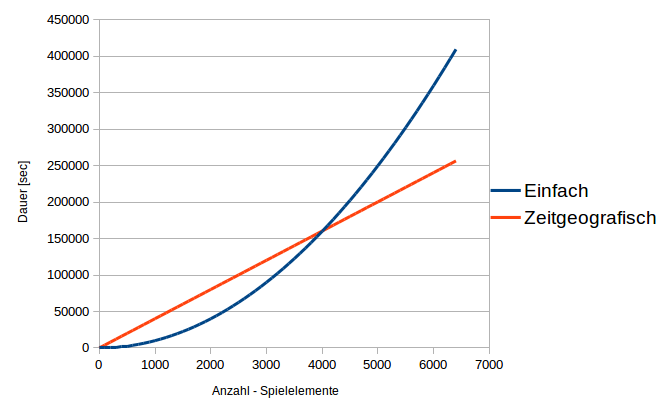
\includegraphics[width=150mm]{images/ch6_img05_eval_match.png}
\caption{Gegenüberstellung der cNN Methoden}
\label{img:ch6_img05_eval_match}
\end{center}
\end{figure}

Allerdings muss beachtet werden, dass bei 4100 Spielelementen auf 6,25km$^2$, eine extrem hohe Dichte erreicht wird. Diese führt dazu, dass es im Schnitt es weniger als 40 Meter bis zum nächsten Spielelement sind. Bei einem Aktionsradius von 40 Metern, wäre das Spielfeld somit voller Spielelemente. Daraus folgern sich zwei Dinge:
Die ideale Spielelementzahl sollte einen Flächen zu Spielemement Index größer als 1524m$^2$ aufweisen.
Es ist auch festzustellen, dass der Einsatz der zeitgeographische Methode keinen Sinn macht.
Nachdem die Berechnungsmethode festgelegt wurde und die Werte für verschiedene Punkte berechnet wurde, wurde festgestellt, dass ein Clustering sich nicht negativ auf die Ergebnisse auswirkt.
Der Grund hierfür liegt in der Bewertungsfunktion. Jedes Spielelement im Bereich von 0 bis 700 Meter wird als ein nächster Nachbar gezählt.
Die Ursprüngliche Vorgehensweise hatte als Bewertungsfunktion der einzelnen Tags:

\begin{equation}
score = \frac{ \sum\limits_{i=1}^n c_n }{n}
\end{equation}

Um dieses Problem zu umgehen muss eine Bewertungsfunktion für die unterschiedlichen Entfernungen erstellt werden. Ein erster Ansatz die Verwendung einer Gleichung zweiter Ordnung wie in Abbildung \ref{img:ch6_img06_valued2} zu erkennen. Nach einem ersten Probelauf hat sich allerdings herausgestellt, dass die Elemente im Bereich von unter 1000 Metern zu schwach negativ ins Gewicht fallen.

\begin{figure}[H]
\begin{center}
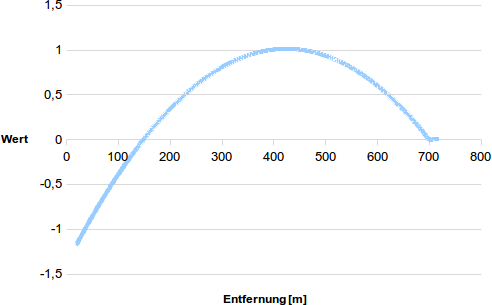
\includegraphics[width=150mm]{images/ch6_img06_valued2.png}
\caption{Bewertungsfunktion für Distanzen}
\label{img:ch6_img06_valued2}
\end{center}
\end{figure}

\begin{equation}
weighted score = \frac{ \sum\limits_{i=1}^n cv_n }{n}
\end{equation}

Aus diesem Grund wurde auf eine abgestufte Bewertung gewechselt, welche das Ergebnis für die entsprechenden Tags besser normalisiert hat.
Allerdings ist das Ergebnis welches in Abbildung \ref{img:ch6_img07_result1} zu sehen ist noch nicht das Optimum. Es wird daher vorgeschlagen, die Bewertungsfunktion weiter zu optimieren und Ansätze aus der Fuzzy Logic zu verfolgen, da diese eine deutlich bessere Steuerung der einzelnen Attribute und Entfernungen ermöglichen. Eine vollständige Grafik aller Werte ist im Anhang zu finden. Die in Abbildung \ref{img:ch6_img07_result1} gezeigte Darstellung zeigt die Tags die weniger als 70 Nachbar-Elemente im Umkreis von 700 Metern haben.
Es lässt sich erkennen, dass Elemente, welche durch die Infrastruktur bedingt verteilt gelegen sind wie z.B: Bushaltestellen, Bäckereien und Ampel eine bessere Verteilung haben als zum Beispiel Schulen. Allerdings muss beachtet werden, dass allein durch ein höheren Wert nicht sichergestellt ist, dass der Tag überall gut funktioniert. Viel wichtiger dabei ist der Abgleich der Werte aus verschiedenen Regionen. Erst mit dem Vergleich der Ergebnisse der einzelnen Tags an unterschiedlichen Orten, an denen ein Staging stattfinden soll, ermöglicht eine Auswahl.
Der Tag, welcher bei allen Überprüften Lokalitäten den ausgeglichensten Wert hat, sollte verwendet werden. Gibt es mehrere Tags die im Schnitt wenig voneinander Abweichen, sollte der Tag mit dem höchsten Wert verwendet werden. 

\begin{figure}[H]
\begin{center}
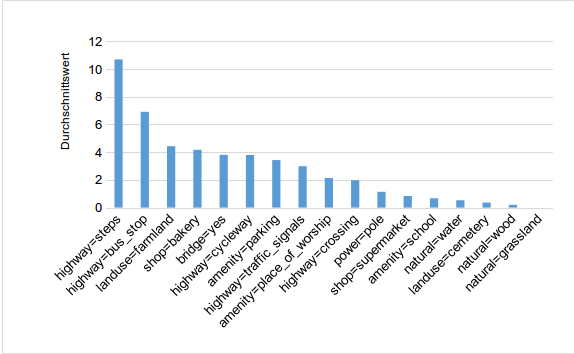
\includegraphics[width=150mm]{images/ch6_img07_result1.png}
\caption{Bewertung der einzelnen Tags}
\label{img:ch6_img07_result1}
\end{center}
\end{figure}

\newpage
\chapter{Diskussion}
\label{sec:S7_Diskussion}

\section{Relokalisierbarkeit geobasierter Gamification-Ansätze}

Nach der Evaluation des Frameworks und des Beispielspiels kann festgehalten werden, dass die zuvor in der Problemstellung geschilderten Anforderungen mit Hilfe des beschriebenen Frameworks gelöst werden können. Um der Echtzeitanforderung gerecht zu werden, wurde die Auswahl der Spielelemente anhand von OSM-Daten auf eine zweistufiges Verfahren ausgelegt. Der ressourcenaufwendigere Part wurde ausgegliedert und vor das Pervasive Game gestellt. Hierzu wurde ein Evaluationstool entwickelt welches anhand einer gegebenen Position und eines Key-Value Paars die Spielfläche automatisch bewertet und für einen Vergleich mit anderen Spielfeldern herangezogen werden kann.
Die Auswahl wiederum kann im Framework entsprechend festgehalten werden. Es wurde festgestellt, dass gewisse Stellen weiter einer Optimierung bedürfen um noch bessere Ergebnisse zu erzielen. Hierunter fällt die Bewertung der Entfernungsmatrix welche für die einzelnen Spielelemente der Transformation erzeugt wird. Erste Ansätze und Ergebnisse wurden entsprechend geschildert, sowie weitere Vorgehensweisen präsentiert.
Es wurde eine funktionierende Transformation für die Umwandlung von OSM-Elementen zu Spielelementen entworfen und entsprechend umgesetzt.
Basierend auf der Transformation wurde eine entsprechende Schnittstelle entworfen, die es ermöglicht, sowohl für das darauf aufbauende Spiel, als auch für die Administration und die Evaluierung der Tags entsprechend die GeoDaten aufzubereiten.
\\\\
Die Untersuchungen haben ergeben, dass eine Realisierbarkeit mit Hilfe von OSM-Daten möglich ist. Hierfür muss im gewählten Fall eine Vorselektion anhand der Tags stattfinden, um die Evaluation der Spielfelder auszulagern. Mit dem Transformationsprozess in Kombination des vorgestellten Frameworks konnte gezeigt werden, dass OSM Daten Problemlos nutzbar sind. Durch den beschriebenen Lösungsansatz wird ein entsprechender Beitrag zur Untersuchung von Möglichkeiten zur automatischen/unterstützen Erstellung von Spielfeldern geleistet. Dadurch ist es möglich auf Basis der vorgestellten Lösung weitere Optimierungen der Ansätze durchzuführen. 

\section{Ausblick}

Durch die Untersuchung haben sich mehrere Punkte ergeben die zu hinterfragen und zu evaluieren sind. Zunächst ist die Evaluation der Spielfelder zu nennen. Hierbei wurden erste Ansätze aufgezeigt und entsprechend optimiert. Durch die Vorausstellung der Evaluation der OSM-Tags und der damit verbundenen Spielfelder bietet diese den Kompromiss der Echtzeit Generierung der Spielfelder. Nichtsdestotrotz ist eine weitere Verbesserung der Bewertung der Spielfelder erstrebenswert um noch besser auf die Effekte des Clusterings eingehen zu können. Oder im Idealfall diese zu vermeiden. Hierbei sollte dem Spielleiter auch mehr Flexibilität an die Hand gelegt werden, um auch die gewünschten Abstände einzustellen. Im Moment ist die maximale Entfernung bei der Bewertung bei 700 Meter und es wird eine mindest- Entfernung von 150 Metern  mathematisch bevorzugt. Hierbei handelt es sich nicht um wissenschaftlich untersuchte Werte sondern um eine erste festgelegte Kenngröße.
Damit verbunden ist eine Evaluation der Spielfelder bei realen Spielern. Dieses Feedback ist unerlässlich für eine weitere Optimierung des Frameworks. Dies könnte auf Basis einer optisch aufgewertete Version des Beispielspiels passieren, wodurch der Aufwand für eine Evaluation gering gehalten wird.
Hierbei ist es zu empfehlen eine iterative Vorgehensweise zu nutzen um entsprechendes Feedback in den Tests entsprechend in das Framework einfließen zu lassen.
Ein weiterer offener Punkt stellt die Skalierbarkeit des Frameworks dar. Zwar wurden die Abfrage Zeiten entsprechend Optimiert, genauere Untersuchungen im Hinblick auf Last und konkreter Ressourcenverbrauch stehen allerdings aus. Interssant wäre hierbei zu untersuchen, wie viele Spieler maximal bedient werden können mit einer festen Größe an Ressourcen. Hierbei sollte auch untersucht werden, inwiefern ein entsprechendes Caching der Transformation von Nöten ist. In Kapitel XX wurde das Caching bereits angesprochen. Sofern dies im Zuge der Skalierbarkeit angegangen wird, muss ein detaillierter Ansatz für das Caching entworfen und umgesetzt werden. 
Diese Untersuchungen sind essentiell für den Einsatz eines solchen Frameworks für den Produktivbetrieb.
Der Aspekt der Händler Integration wirft ebenfalls eine Frage auf. Es gibt bisher keine fundierten Untersuchungen bezüglich der Interaktion von (online) Spielern mit der physischen Welt. Es wurden verschiedenen Lösungen zur Interaktion vorgestellt (Coupon, QR-Code, NFC, iBeacon), allerdings gilt es zu untersuchen, welche der Methoden für einen konkreten Einsatz geeignet sind. Hierbei spielen Zielgruppe und die Verbreitung der Technologien eine entscheidende Rolle.
\newpage
\chapter{Glossar}

%\newpage{Abkrzugsverzeichnis}
%\addcontentsline{toc}{chapter}{Abkrzungsverzeichnis}
%%\addcontentsline{toc}{chapter}{\protect{Glossar}}
\begin{acronym}[abkuerzungen2]
\acro{API}{Die API stellt eine dokumentierte Software-Schnittstelle dar, die von anderen Programmen aus genutzt werden kann.}
\acro{Basismaschine}{Eine Basismaschine stellt Datenobjekte und Operatoren bereit, auf deren Grundlage die Datenobjekte und Operatoren der Nutzermaschine realisiert werden.}
\acro{CLI}{Command Line Interface - Kommandozeile. Die Kommandozeile ist ein Eingabebereich für die Steuerung einer Software, die typischerweise im Textmodus abläuft.}
\acro{DNS}{Ermöglicht es Klarnamen in numerische IP Adressen (z.B. google-public-dns-a.google.com in 8.8.8.8 umzuwandeln).}
\acro{GUI}{Hierbei handelt es sich um die grafische Benutzeroberfläche.}
\acro{RFC}{RFCs sind eine Reihe von technischen und organisatorischen Dokumenten zum Internet, die sie zu einem Standard entwickelt haben.}
\acro{POI}{Pointn of Interest. Sehenswürdigkeit}
\acro{PBL}{Points, Badgets, Leaderboards}
\acro{Shell}{Eingabe-Schnittstelle zwischen Computer und Benutzer}
\acro{SQL}{Eine deskriptive Abfragesprache von Datenbanken.}
\end{acronym}

\newpage
%% - alphadin
%%\bibliography{references}
\nocite{*} 
\printbibliography[heading=bibintoc]
\newpage

\chapter{Eidestattliche Erklärung}
\label{sec:S9_Eid}

\newpage

\end{document}
